% Problems, Chapter 9: Radiating Systems, Multipole Fields and Radiation
% Jackson, Classical Electrodynamics, 3rd ed.
% Requires: amsmath, amssymb, tikz

\section*{Problems}

\Needspace{5\baselineskip}
\par\bigskip
\noindent\textbf{9.1}\quad A common textbook example of a radiating system (see Problem 9.2) is a configuration of charges fixed relative to each other but in rotation. The charge density is obviously a function of time, but it is not in the form of (9.1).
\begin{enumerate}
\item[(a)] Show that for rotating charges one alternative is to calculate \emph{real} time-dependent multipole moments using $\rho(\mathbf{x},t)$ directly and then compute the multipole moments for a given harmonic frequency with the convention of (9.1) by inspection or Fourier decomposition of the time-dependent moments. Note that care must be taken when calculating $q_{lm}(t)$ to form linear combinations that are real before making the connection.
\item[(b)] Consider a charge density $\rho(\mathbf{x},t)$ that is periodic in time with period $T=2\pi/\omega_{0}$. By making a Fourier \emph{series} expansion, show that it can be written as
\[
\rho(\mathbf{x},t)=\rho_{0}(\mathbf{x})+\sum_{n=1}^{\infty}\mathrm{Re}[2\rho_{n}(\mathbf{x})e^{-in\omega_{0}t}]
\]
where
\[
\rho_{n}(\mathbf{x})=\frac{1}{T}\int_{0}^{T}\rho(\mathbf{x},t)e^{in\omega_{0}t}\;dt
\]
This shows explicitly how to establish connection with (9.1).
\item[(c)] For a single charge $q$ rotating about the origin in the $x$-$y$ plane in a circle of radius $R$ at constant angular speed $\omega_{0}$, calculate the $l=0$ and $l=1$ multipole moments by the methods of parts a and b and compare. In method b express the charge density $\rho_{n}(\mathbf{x})$ in cylindrical coordinates. Are there higher multipoles, for example, quadrupole? At what frequencies?
\end{enumerate}
\solution

Use $Y_{lm}=N_{lm}P_l^m(\cos\theta)e^{im\phi}$ with the
Condon--Shortley phase, with
$N_{lm}=[(2l+1)(l-m)!/(4\pi(l+m)!)]^{1/2}$.
We use $q_{lm}(t)=\int r^lY_{lm}^*\rho(\mathbf x,t)d^3x$ for the
instantaneous complex spherical moment, and Jackson's $Q_{lm}$ for
its electric source phasor at a specified positive frequency.
A phasor below means the coefficient inside
$\operatorname{Re}[\cdots e^{-i\Omega t}]$, not a two-sided Fourier coefficient.

\textbf{(a)} Multipole formation is linear. Thus for every real Cartesian
moment $F(t)$, Fourier expansion commutes with the spatial integral defining
$F$. In particular, expand $p_x,p_y,p_z$ or the five real components of
$Q_{ij}$, and then convert their phasors to spherical components. A complex
quantity such as $q_{11}(t)=-\sqrt{3/(8\pi)}[p_x(t)-ip_y(t)]$ is not itself a
real observable; taking its real part before this conversion loses information.

\textbf{(b)} Orthogonality of $e^{in\omega_0t}$ gives
\[
\rho=\sum_{n=-\infty}^{\infty}\rho_ne^{-in\omega_0t},\qquad
\rho_n=T^{-1}\int_0^T\rho e^{in\omega_0t}dt.
\]
Reality gives $\rho_{-n}=\rho_n^*$, so pairing $n$ with $-n$ yields exactly
$\rho_0+\sum_{n\ge1}\operatorname{Re}[2\rho_ne^{-in\omega_0t}]$.
Consequently the positive-frequency source phasor is $2\rho_n$.

\textbf{(c)} Write cylindrical radius as $s$ and use the periodic delta
$\delta_{2\pi}$. Then
\[
\rho=\frac q{s}\delta(s-R)\delta(z)\delta_{2\pi}(\phi-\omega_0t),
\qquad
\boxed{\rho_n=\frac q{2\pi s}\delta(s-R)\delta(z)e^{in\phi}.}
\]
Directly, the real moments are
\[
q_{00}=\frac q{\sqrt{4\pi}},\quad
\mathbf p(t)=qR(\hat{\mathbf x}\cos\omega_0t+
\hat{\mathbf y}\sin\omega_0t),\quad q_{10}=0.
\]
Thus $\mathbf p_{\omega_0}=qR(\hat{\mathbf x}+i\hat{\mathbf y})$,
$(Q_{11})_{\omega_0}=-2qR\sqrt{3/(8\pi)}$, and
$(Q_{1,-1})_{\omega_0}=0$.
Alternatively direct integration of $\rho_n$ gives
\[
\int r^lY_{lm}^*\rho_n\,d^3x
=qR^lY_{lm}^*(\pi/2,0)\delta_{mn}.
\]
Doubling this for $n>0$ reproduces the preceding phasors. Before taking a
phasor, the complex time-dependent moments themselves are
$q_{11}(t)=-qR\sqrt{3/(8\pi)}e^{-i\omega_0t}$ and
$q_{1,-1}(t)=qR\sqrt{3/(8\pi)}e^{i\omega_0t}$; this displays the factor-of-two
trap in part (a).

All $l,m$ for which $P_l^m(0)\ne0$ occur: $l+m$ must be even. The $m=0$
terms are static, while $|m|>0$ terms oscillate at $|m|\omega_0$.
For example $q_{20}=-qR^2\sqrt{5/(16\pi)}$ is static and
$q_{22}=qR^2\sqrt{15/(32\pi)}e^{-2i\omega_0t}$, with its reality-related
$m=-2$ partner, supplies electric quadrupole radiation at $2\omega_0$.

\Needspace{5\baselineskip}
\par\bigskip
\noindent\textbf{9.2}\quad A radiating quadrupole consists of a square of side $a$ with charges $\pm q$ at alternate corners. The square rotates with angular velocity $\omega$ about an axis normal to the plane of the square and through its center. Calculate the quadrupole moments, the radiation fields, the angular distribution of radiation, and the total radiated power, all in the long-wavelength approximation. What is the frequency of the radiation?
\solution

Choose the positive charges initially at $\pm R\hat{\mathbf x}$ and the
negative charges at $\pm R\hat{\mathbf y}$, where $R=a/\sqrt2$. A change
of the initial orientation changes only phases. The net charge, electric
dipole and magnetic dipole vanish. With $\Omega=2\omega$, direct summation
of $Q_{ij}=\sum_s q_s(3x_{si}x_{sj}-r_s^2\delta_{ij})$ gives
\[
Q(t)=3qa^2\begin{pmatrix}
\cos\Omega t&\sin\Omega t&0\\
\sin\Omega t&-\cos\Omega t&0\\0&0&0
\end{pmatrix},\qquad
\mathcal Q=3qa^2\begin{pmatrix}1&i&0\\i&-1&0\\0&0&0\end{pmatrix}.
\]
Thus the positive-frequency spherical moment is only
$Q_{22}=qa^2\sqrt{15/(2\pi)}$. Put $K=\Omega/c$ and
$\mathbf v=\mathcal Q\mathbf n$. The radiation fields are
\[
\boxed{\mathbf E=-\frac{iK^3}{24\pi\epsilon_0}
 [\mathbf v-\mathbf n(\mathbf n\cdot\mathbf v)]\frac{e^{iKr}}r,
\qquad \mathbf H=\frac1{Z_0}\mathbf n\times\mathbf E.}
\]
These follow by expanding the retarded vector potential to first order
in the source coordinate and using continuity: its symmetric part is
$\mathbf A_Q=-\mu_0cK^2\mathcal Q\mathbf n\,e^{iKr}/(24\pi r)$;
$\mathbf E_T=i\Omega\mathbf A_T$.
Explicitly, if $A=3qa^2$,
$\mathbf v=A\sin\theta e^{i\phi}(\hat{\mathbf x}+i\hat{\mathbf y})$,
so $|\mathbf v|^2=2A^2\sin^2\theta$ and
$|\mathbf n\cdot\mathbf v|^2=A^2\sin^4\theta$. Therefore
\[
\boxed{\frac{d\overline P}{d\Omega}
=\frac{cq^2a^4K^6}{128\pi^2\epsilon_0}(1-\cos^4\theta).}
\]
Since $2\pi\int_{-1}^1(1-u^4)du=16\pi/5$,
\[
\boxed{\overline P=\frac{cq^2a^4K^6}{40\pi\epsilon_0}
=\frac{8q^2a^4\omega^6}{5\pi\epsilon_0c^5},\qquad
\Omega=2\omega.}
\]
The physical fields are the real parts after multiplication by
$e^{-i\Omega t}$; the square returns to the same charge configuration
after half a revolution.

\Needspace{5\baselineskip}
\par\bigskip
\noindent\textbf{9.3}\quad Two halves of a spherical metallic shell of radius $R$ and infinite conductivity are separated by a very small insulating gap. An alternating potential is applied between the two halves of the sphere so that the potentials are $\pm V\cos\omega t$. In the long-wavelength limit, find the radiation fields, the angular distribution of radiated power, and the total radiated power from the sphere.
\solution

Take the gap in the equatorial plane. In the quasistatic exterior solution
write $\Phi(R,\theta)=V\,\operatorname{sgn}(\cos\theta)$ for its phasor.
Its $l=1$ Legendre coefficient is
\[
A_1=\frac32\int_{-1}^1Vu\,\operatorname{sgn}u\,du=\frac32V.
\]
Thus $\Phi_1=(3VR^2/2r^2)\cos\theta$ and comparison with
$\Phi_p=p\cos\theta/(4\pi\epsilon_0r^2)$ gives
$\mathbf p=6\pi\epsilon_0VR^2\hat{\mathbf z}$.
Higher odd electric multipoles are smaller in radiated amplitude by
successive powers of $(kR)^2$. The leading radiation is
\[
E_\theta=-\frac32Vk^2R^2\sin\theta\frac{e^{ikr}}r,
\qquad H_\phi=E_\theta/Z_0,
\]
with all other radiation components zero. Consequently
\[
\boxed{\frac{d\overline P}{d\Omega}
=\frac98\epsilon_0cV^2k^4R^4\sin^2\theta,
\qquad \overline P=3\pi\epsilon_0cV^2k^4R^4.}
\]
Here the voltage difference is $2V$, not $V$, and
$\int\sin^2\theta\,d\Omega=8\pi/3$.

\Needspace{5\baselineskip}
\par\bigskip
\noindent\textbf{9.4}\quad Apply the approach of Problem 9.1b to the current and magnetization densities of the particle of charge $q$ rotating about the origin in the $x$-$y$ plane in a circle of radius $R$ at constant angular speed $\omega_{0}$. The motion is such that $\omega_{0}R\ll c$.
\begin{enumerate}
\item[(a)] Find $(J_{x})_{n}$, $(J_{y})_{n}$, and $(J_{z})_{n}$ in terms of cylindrical coordinates for all $n$. Also determine the components of the orbital ``magnetization,'' $(\mathbf{x}\times\mathbf{J}_{n})/2$, and its divergence [which plays the role of a magnetic charge density for magnetic multipoles, as in $M_{lm}$ (9.172)].
\item[(b)] What long-wavelength magnetic multipoles $(l,m)$ occur and at what frequencies? [Remember that the multipole order $l$ does not necessarily equal the harmonic number $n$.]
\item[(c)] Use linear superposition to generalize your argument to the four charges rotating in Problem 9.2 at radius $R=a/\sqrt{2}$. What harmonics occur, and what magnetic multipoles at each harmonic? Is there a magnetic multipole contribution at the $E2$ frequency of Problem 9.2? Is it significant relative to the $E2$ radiation?
\end{enumerate}
\solution

\textbf{(a)} The particle velocity at its position is
$\omega_0s\hat{\boldsymbol\phi}$. Multiplication of the Fourier density
in 9.1 therefore gives, for every integer $n$,
\[
\mathbf J_n=\frac{q\omega_0}{2\pi}\delta(s-R)\delta(z)e^{in\phi}
\hat{\boldsymbol\phi}.
\]
Its Cartesian components are this scalar times $(-\sin\phi,\cos\phi,0)$.
The apparent extra harmonics in these components are not extra temporal
frequencies; the cylindrical basis itself depends on position.
On the support $z=0$,
\[
\mathcal M_n=\tfrac12\mathbf x\times\mathbf J_n
=\frac{q\omega_0s}{4\pi}\delta(s-R)\delta(z)e^{in\phi}\hat{\mathbf z},
\quad
\nabla\cdot\mathcal M_n
=\frac{q\omega_0s}{4\pi}\delta(s-R)\delta'(z)e^{in\phi}.
\]
The vanishing distribution $z\delta(z)$ in the transverse component
makes no further contribution.

\textbf{(b)} The orbital moment convention of (9.172) is
$M_{lm}=-(2/(l+1))\int r^lY_{lm}^*\nabla\cdot\mathcal M\,d^3x$.
Integrating by parts in $z$ and then integrating $\phi$ gives the
\emph{Fourier coefficient}
\[
\boxed{(M_{lm})_n=\frac{q\omega_0R^{l+1}}{l+1}
N_{lm}(P_l^m)'(0)\delta_{mn}.}
\]
In obtaining this expression use
$\partial_z[r^lP_l^m(z/r)]_{z=0}=R^{l-1}(P_l^m)'(0)$.
It is nonzero only when $l+m$ is odd. For $n>0$ the phasor is twice
this expression: the allowed magnetic multipoles are
$m=n$, $l=n+1,n+3,\ldots$, at frequency $n\omega_0$.
The $n=0$ moments have odd $l$ and are static; in particular
$m_z=q\omega_0R^2/2$. Negative-frequency components are fixed by reality.

\textbf{(c)} Superposition adds the phase factor
\[
\sum_{j=0}^3(-1)^je^{-in\pi j/2}
=\begin{cases}4,&n=2\pmod4,\\0,&\text{otherwise}.\end{cases}
\]
Thus the positive harmonics are $n=2,6,10,\ldots$; at each one the
magnetic orders are $l=n+1,n+3,\ldots$, $m=n$.
There is an $M3$ contribution at the $E2$ frequency $2\omega_0$.
For example the leading phasors satisfy
\[
\frac{M_{32}}{Q_{22}}=\frac{\sqrt7}{4}\omega_0R^2.
\]
The general powers are proportional to
$k^{2l+2}[(l+1)/l]|Q_{lm}|^2/[(2l+1)!!]^2$, with
$Q\mapsto M/c$ for magnetic radiation. At $k=2\omega_0/c$ their ratio is
\[
\boxed{\frac{P_{M3}}{P_{E2}}
=\frac{k^2}{c^2}\frac{8}{9}\frac1{49}
\left|\frac{M_{32}}{Q_{22}}\right|^2
=\frac{2}{63}\left(\frac{\omega_0R}{c}\right)^4.}
\]
It is negligible in the stated nonrelativistic limit, despite occurring
at the same frequency.

\Needspace{5\baselineskip}
\par\bigskip
\noindent\textbf{9.5}\quad\begin{enumerate}
\item[(a)] Show that for harmonic time variation at frequency $\omega$ the electric dipole scalar and vector potentials in the Lorenz gauge and the long-wavelength limit are
\begin{gather*}
\Phi(\mathbf{x})=\frac{e^{ikr}}{4\pi\epsilon_{0}r^{2}}\,\mathbf{n}\cdot\mathbf{p}(1-ikr)\\[4pt]
\mathbf{A}(\mathbf{x})=-i\,\frac{\mu_{0}\omega}{4\pi}\frac{e^{ikr}}{r}\,\mathbf{p}\qquad\text{[this is (9.16)]}
\end{gather*}
where $k=\omega/c$, $\mathbf{n}$ is a unit vector in the radial direction, $\mathbf{p}$ is the dipole moment (9.17), and the time dependence $e^{-i\omega t}$ is understood.
\item[(b)] Calculate the electric and magnetic fields \emph{from the potentials} and show that they are given by (9.18).
\end{enumerate}
\solution

\textbf{(a)} Expand the outgoing Helmholtz Green function for a localized
source:
\[
\frac{e^{ik|\mathbf x-\mathbf x'|}}{|\mathbf x-\mathbf x'|}
=\frac{e^{ikr}}r-\mathbf x'\cdot\nabla\frac{e^{ikr}}r+\cdots.
\]
The electric dipole part of the scalar potential is consequently
$\Phi_p=-(4\pi\epsilon_0)^{-1}\mathbf p\cdot\nabla(e^{ikr}/r)$.
Since $\nabla(e^{ikr}/r)=\mathbf n e^{ikr}(ik/r-1/r^2)$, this is the
stated scalar potential. Integrating
$\nabla'\cdot\mathbf J=i\omega\rho$ against $x'_i$ gives
$\int J_i\,d^3x'=-i\omega p_i$; the zeroth spatial moment of the vector
potential is therefore
$\mathbf A=-i\mu_0\omega\mathbf p\,e^{ikr}/(4\pi r)$.
A time-independent net charge, if present, has its separate Coulomb field.

\textbf{(b)} Define $f(r)=e^{ikr}/r$. Then
\[
\mathbf B=\nabla\times\mathbf A
=-\frac{i\mu_0\omega}{4\pi}f'\mathbf n\times\mathbf p
=\frac{\mu_0c}{4\pi}e^{ikr}
\left(\frac{k^2}{r}+\frac{ik}{r^2}\right)\mathbf n\times\mathbf p.
\]
For the electric field use
$\partial_i\partial_j f=(f''-f'/r)n_in_j+(f'/r)\delta_{ij}$ and
\[
f'=e^{ikr}(ik/r-1/r^2),\qquad
f''=e^{ikr}(-k^2/r-2ik/r^2+2/r^3).
\]
Then $\mathbf E=-\nabla\Phi+i\omega\mathbf A$ gives
\[
\boxed{\mathbf E=\frac{e^{ikr}}{4\pi\epsilon_0}
\left\{\frac{k^2}{r}[(\mathbf n\times\mathbf p)\times\mathbf n]
+\left(\frac1{r^3}-\frac{ik}{r^2}\right)
[3\mathbf n(\mathbf n\cdot\mathbf p)-\mathbf p]\right\},}
\]
\[
\boxed{\mathbf H=\frac{ck^2}{4\pi}\frac{e^{ikr}}r
\left(1+\frac{i}{kr}\right)\mathbf n\times\mathbf p.}
\]
These retain the electrostatic, induction and radiation fields while
keeping only the electric dipole source moment.

\Needspace{5\baselineskip}
\par\bigskip
\noindent\textbf{9.6}\quad\begin{enumerate}
\item[(a)] Starting from the general expression (9.2) for $\mathbf{A}$ and the corresponding expression for $\Phi$, expand both $R=|\mathbf{x}-\mathbf{x}'|$ and $t'=t-R/c$ to first order in $|\mathbf{x}'|/r$ to obtain the electric dipole potentials for arbitrary time variation
\begin{gather*}
\Phi(\mathbf{x},t)=\frac{1}{4\pi\epsilon_{0}}\left[\frac{1}{r^{2}}\,\mathbf{n}\cdot\mathbf{p}_{\mathrm{ret}}+\frac{1}{cr}\,\mathbf{n}\cdot\frac{\partial\mathbf{p}_{\mathrm{ret}}}{\partial t}\right]\\[4pt]
\mathbf{A}(\mathbf{x},t)=\frac{\mu_{0}}{4\pi r}\frac{\partial\mathbf{p}_{\mathrm{ret}}}{\partial t}
\end{gather*}
where $\mathbf{p}_{\mathrm{ret}}=\mathbf{p}(t'=t-r/c)$ is the dipole moment evaluated at the retarded time measured from the origin.
\item[(b)] Calculate the dipole electric and magnetic fields directly from these potentials and show that
\begin{gather*}
\mathbf{B}(\mathbf{x},t)=\frac{\mu_{0}}{4\pi}\left[-\frac{1}{\erratum{r^{2}}}\,\mathbf{n}\times\frac{\partial\mathbf{p}_{\mathrm{ret}}}{\partial t}-\frac{1}{\erratum{cr}}\,\mathbf{n}\times\frac{\partial^{2}\mathbf{p}_{\mathrm{ret}}}{\partial t^{2}}\right]\\[4pt]
\mathbf{E}(\mathbf{x},t)=\frac{1}{4\pi\epsilon_{0}}\left\{\left(1+\frac{r}{c}\frac{\partial}{\partial t}\right)\!\left[\frac{3\mathbf{n}(\mathbf{n}\cdot\mathbf{p}_{\mathrm{ret}})-\mathbf{p}_{\mathrm{ret}}}{r^{3}}\right]+\frac{1}{c^{2}r}\,\mathbf{n}\times\!\left(\mathbf{n}\times\frac{\partial^{2}\mathbf{p}_{\mathrm{ret}}}{\partial t^{2}}\right)\right\}
\end{gather*}
\item[(c)] Show explicitly how you can go back and forth between these results and the harmonic fields of (9.18) by the substitutions $-i\omega\leftrightarrow\partial/\partial t$ and $\mathbf{p}e^{ikr-i\omega t}\leftrightarrow\mathbf{p}_{\mathrm{ret}}(t')$.
\end{enumerate}
\solution

\textbf{(a)} Put $t_r=t-r/c$. To first order in the source coordinate,
\[
R=r-\mathbf n\cdot\mathbf x'+\cdots,\quad
R^{-1}=r^{-1}+r^{-2}\mathbf n\cdot\mathbf x'+\cdots,\quad
\rho(\mathbf x',t-R/c)=\rho(\mathbf x',t_r)
+\frac{\mathbf n\cdot\mathbf x'}c\dot\rho(\mathbf x',t_r)+\cdots.
\]
Integrate their product in the retarded scalar potential. Its dipole
terms are $\mathbf n\cdot\mathbf p/r^2+
\mathbf n\cdot\dot{\mathbf p}/(cr)$, divided by $4\pi\epsilon_0$.
The omitted monopole is the constant total charge divided by
$4\pi\epsilon_0r$. Integration of the continuity equation times $x'_i$
gives $\int J_i\,d^3x'=\dot p_i$, so the dipole vector potential is
$\mu_0\dot{\mathbf p}(t_r)/(4\pi r)$ as claimed. This source expansion
also requires the source light-crossing time to be short compared with
its variation time; $r$ itself need not be in the radiation zone.

\textbf{(b)} All time derivatives below are at $t_r$. The identities
\[
\partial_i t_r=-n_i/c,\qquad
\partial_i n_j=(\delta_{ij}-n_in_j)/r
\]
ensure that spatial differentiation includes retardation. In particular
\[
\nabla\frac{\mathbf n\cdot\mathbf p}{r^2}
=\frac{\mathbf p-3\mathbf n(\mathbf n\cdot\mathbf p)}{r^3}
-\frac{\mathbf n(\mathbf n\cdot\dot{\mathbf p})}{cr^2},
\]
\[
\nabla\frac{\mathbf n\cdot\dot{\mathbf p}}{cr}
=\frac{\dot{\mathbf p}-2\mathbf n(\mathbf n\cdot\dot{\mathbf p})}{cr^2}
-\frac{\mathbf n(\mathbf n\cdot\ddot{\mathbf p})}{c^2r}.
\]
Adding $-\partial_t\mathbf A=-\ddot{\mathbf p}/(4\pi\epsilon_0c^2r)$
to minus these gradients gives
\[
\boxed{\mathbf E=\frac1{4\pi\epsilon_0}\left[
\frac{3\mathbf n(\mathbf n\cdot\mathbf p)-\mathbf p}{r^3}
+\frac{3\mathbf n(\mathbf n\cdot\dot{\mathbf p})-\dot{\mathbf p}}{cr^2}
+\frac{\mathbf n\times(\mathbf n\times\ddot{\mathbf p})}{c^2r}\right].}
\]
Curling $\dot{\mathbf p}(t_r)/r$ gives separately the derivative of $1/r$
and that of its retarded argument:
\[
\boxed{\mathbf B=-\frac{\mu_0}{4\pi}\left[
\frac{\mathbf n\times\dot{\mathbf p}}{r^2}
+\frac{\mathbf n\times\ddot{\mathbf p}}{cr}\right].}
\]
This also confirms the two corrected radial powers in the question.

\textbf{(c)} For $\mathbf p(t_r)=\mathbf p_0e^{-i\omega(t-r/c)}$,
$\dot{\mathbf p}=-i\omega\mathbf p$ and
$\ddot{\mathbf p}=-\omega^2\mathbf p$. Substitution in the last two
expressions gives the two boxed harmonic fields in 9.5 after removing
$e^{-i\omega t}$. Conversely each power of $-i\omega$ in those fields
becomes a time derivative under Fourier superposition. This applies to
arbitrary sufficiently differentiable source histories, not only a
single sinusoid.

\Needspace{5\baselineskip}
\par\bigskip
\noindent\textbf{9.7}\quad\begin{enumerate}
\item[(a)] By means of Fourier superposition of different frequencies or equivalent means, show for a real electric dipole $\mathbf{p}(t)$ that the instantaneous radiated power per unit solid angle at a distance $r$ from the dipole in a direction $\mathbf{n}$ is
\[
\frac{dP(t)}{d\Omega}=\frac{Z_{0}}{16\pi^{2}c^{2}}\left|\left[\mathbf{n}\times\frac{d^{2}\mathbf{p}}{dt'^{2}}(t')\right]\times\mathbf{n}\right|^{2}
\]
where $t'=t-r/c$ is the retarded time. For a magnetic dipole $\mathbf{m}(t)$, substitute $(1/c)\ddot{\mathbf{m}}\times\mathbf{n}$ for $(\mathbf{n}\times\ddot{\mathbf{p}})\times\mathbf{n}$.
\item[(b)] Show similarly for a real quadrupole tensor $Q_{\alpha\beta}(t)$ given by (9.41) with a real charge density $\rho(\mathbf{x},t)$ that the instantaneous radiated power per unit solid angle is
\[
\frac{dP(t)}{d\Omega}=\frac{Z_{0}}{576\pi^{2}c^{4}}\left|\left[\mathbf{n}\times\frac{d^{3}\mathbf{Q}}{dt'^{3}}(\mathbf{n},t')\right]\times\mathbf{n}\right|^{2}
\]
where $\mathbf{Q}(\mathbf{n},t)$ is defined by (9.43).
\end{enumerate}
\solution

\textbf{(a)} The $r^{-1}$ electric field in 9.6 is
$\mathbf E_{\rm rad}=[\mathbf n\times(\mathbf n\times\ddot{\mathbf p})]/
(4\pi\epsilon_0c^2r)$ and
$\mathbf H_{\rm rad}=\mathbf n\times\mathbf E_{\rm rad}/Z_0$.
For real instantaneous fields there is no factor $1/2$ in the Poynting
vector. Hence $dP/d\Omega=r^2|\mathbf E_{\rm rad}|^2/Z_0$, and
$1/(\epsilon_0^2c^4Z_0)=Z_0/c^2$ gives the stated coefficient.
Electric--magnetic duality gives the replacement
$(\mathbf n\times\ddot{\mathbf p})\times\mathbf n
\mapsto\ddot{\mathbf m}\times\mathbf n/c$.

\textbf{(b)} The symmetric first spatial moment of the retarded vector
potential is
\[
( A_Q)_i=\frac{\mu_0}{24\pi cr}n_j\ddot Q_{ij}(t_r)
+\hbox{a longitudinal trace term}.
\]
To see the coefficient, continuity implies
$\int(x_iJ_j+x_jJ_i)d^3x=\partial_t\int x_ix_j\rho\,d^3x$;
the symmetric part is one half of this, and extracting the traceless
quadrupole supplies another factor $1/3$. The retarded spatial expansion
supplies $n_j\partial_t/c$. Taking $-\partial_t\mathbf A_T$ therefore gives
\[
\mathbf E_Q=-\frac{1}{24\pi\epsilon_0c^3r}
\{\mathbf Q^{(3)}(\mathbf n,t_r)
-\mathbf n[\mathbf n\cdot\mathbf Q^{(3)}(\mathbf n,t_r)]\}.
\]
Squaring, multiplying by $r^2/Z_0$, and using
$1/(\epsilon_0^2c^6Z_0)=Z_0/c^4$ proves the second formula.
For a harmonic phasor, time averaging introduces the additional factor
$1/2$ and replaces $\partial_t^3$ by $(-i\omega)^3$, agreeing with 9.2.

\Needspace{5\baselineskip}
\par\bigskip
\noindent\textbf{9.8}\quad\begin{enumerate}
\item[(a)] Show that a classical oscillating electric dipole $\mathbf{p}$ with fields given by (9.18) radiates electromagnetic angular momentum to infinity at the rate
\[
\frac{d\mathbf{L}}{dt}=\frac{k^{3}}{12\pi\epsilon_{0}}\,\mathrm{Im}[\mathbf{p}^{*}\times\mathbf{p}]
\]
\item[(b)] What is the ratio of angular momentum radiated to energy radiated? Interpret.
\item[(c)] For a charge $e$ rotating in the $x$-$y$ plane at radius $a$ and angular speed $\omega$, show that there is only a $z$ component of radiated angular momentum with magnitude $dL_{z}/dt=e^{2}k^{3}a^{2}/6\pi\epsilon_{0}$. What about a charge oscillating along the $z$ axis?
\item[(d)] What are the results corresponding to parts a and b for magnetic dipole radiation?
\end{enumerate}
\emph{Hint}: The electromagnetic angular momentum density comes from more than the transverse (radiation zone) components of the fields.
\solution

\textbf{(a)} Use the outward angular-momentum flux through a sphere,
$-r^3\int\mathbf n\times(\langle T\rangle\cdot\mathbf n)d\Omega$,
where $T$ is the Maxwell stress tensor. Since $B_r=0$ for an electric
dipole, its nonzero contribution is
\[
\dot{\mathbf L}=-\frac{\epsilon_0r^3}{2}
\operatorname{Re}\int E_r^*\,\mathbf n\times\mathbf E_T\,d\Omega.
\]
At large $r$ retain the induction term in the radial field:
\[
E_r=-\frac{2ik}{4\pi\epsilon_0r^2}(
\mathbf n\cdot\mathbf p)e^{ikr}+O(r^{-3}),\qquad
\mathbf n\times\mathbf E_T=
\frac{k^2e^{ikr}}{4\pi\epsilon_0r}\mathbf n\times\mathbf p+O(r^{-2}).
\]
The $r^3$ prefactor cancels these radial powers. Finally,
$\int(\mathbf n\cdot\mathbf p^*)\mathbf n\,d\Omega=(4\pi/3)\mathbf p^*$
gives
\[
\boxed{\dot{\mathbf L}=\frac{k^3}{12\pi\epsilon_0}
\operatorname{Im}(\mathbf p^*\times\mathbf p).}
\]
Dropping the induction field would incorrectly give zero.

\textbf{(b)} Integrating the dipole angular power gives
$\overline P=ck^4|\mathbf p|^2/(12\pi\epsilon_0)$, so
\[
\boxed{\frac{\dot{\mathbf L}}{\overline P}
=\frac1\omega\frac{\operatorname{Im}(\mathbf p^*\times\mathbf p)}{|\mathbf p|^2}.}
\]
For $\mathbf p=\mathbf u+i\mathbf v$ with real vectors,
$\operatorname{Im}(\mathbf p^*\times\mathbf p)=2\mathbf u\times\mathbf v$.
Its magnitude is at most $|\mathbf u|^2+|\mathbf v|^2$; equality holds
for circular polarization. A pure circular dipole carries angular
momentum $\pm\hbar$ along its rotation axis per photon of energy
$\hbar\omega$; linear polarization has zero net angular momentum.

\textbf{(c)} For positive rotation in the $xy$ plane,
$\mathbf p=ea(\hat{\mathbf x}+i\hat{\mathbf y})$, so
$\operatorname{Im}(\mathbf p^*\times\mathbf p)=2e^2a^2\hat{\mathbf z}$.
This gives $\dot L_z=e^2k^3a^2/(6\pi\epsilon_0)$ and no transverse
components. For $\mathbf p=p_0\hat{\mathbf z}$ all components vanish,
although the radiated energy is nonzero.

\textbf{(d)} Duality replaces $\mathbf p$ by $\mathbf m/c$:
\[
\boxed{\dot{\mathbf L}_M=\frac{\mu_0k^3}{12\pi}
\operatorname{Im}(\mathbf m^*\times\mathbf m),\quad
\overline P_M=\frac{\mu_0ck^4}{12\pi}|\mathbf m|^2.}
\]
The ratio is the expression in (b) with $\mathbf p\mapsto\mathbf m$.

\Needspace{5\baselineskip}
\par\bigskip
\noindent\textbf{9.9}\quad\begin{enumerate}
\item[(a)] From the electric dipole fields with general time dependence of Problem 9.6, show that the total power and the total rate of radiation of angular momentum through a sphere at large radius $r$ and time $t$ are
\begin{gather*}
P(t)=\frac{1}{6\pi\epsilon_{0}c^{3}}\left(\frac{\partial^{2}\mathbf{p}_{\mathrm{ret}}}{\partial t^{2}}\right)^{2}\\[4pt]
\frac{d\mathbf{L}_{em}}{dt}=\frac{1}{6\pi\epsilon_{0}c^{3}}\left(\frac{\partial\mathbf{p}_{\mathrm{ret}}}{\partial t}\times\frac{\partial^{2}\mathbf{p}_{\mathrm{ret}}}{\partial t^{2}}\right)
\end{gather*}
where the dipole moment $\mathbf{p}$ is evaluated at the retarded time $t'=t-r/c$.
\item[(b)] The dipole moment is caused by a particle of mass $m$ and charge $e$ moving nonrelativistically in a fixed central potential $V(r)$. Show that the radiated power and angular momentum for such a particle can be written as
\begin{gather*}
P(t)=\frac{\tau}{m}\left(\frac{dV}{dr}\right)^{2}\\[4pt]
\frac{d\mathbf{L}_{em}}{dt}=\frac{\tau}{m}\left(\frac{dV}{r\,dr}\right)\mathbf{L}
\end{gather*}
where $\tau=e^{2}/6\pi\epsilon_{0}mc^{3}$ ($=2e^{2}/3mc^{3}$ in Gaussian units) is a characteristic time, $\mathbf{L}$ is the particle's angular momentum, and the right-hand sides are evaluated at the retarded time. Relate these results to those from the Abraham--Lorentz equation for radiation damping [Section 16.2].
\item[(c)] Suppose the charged particle is an electron in a hydrogen atom. Show that the inverse time defined by the ratio of the rate of angular momentum radiated to the particle's angular momentum is of the order of $\alpha^{4}c/a_{0}$, where $\alpha=e^{2}/4\pi\epsilon_{0}\hbar c\approx1/137$ is the fine structure constant and $a_{0}$ is the Bohr radius. How does this inverse time compare to the observed rate of radiation in hydrogen atoms?
\item[(d)] Relate the expressions in parts a and b to those for harmonic time dependence in Problem 9.8.
\end{enumerate}
\solution

\textbf{(a)} From 9.6 the far electric field has magnitude squared
$[|\ddot{\mathbf p}|^2-(\mathbf n\cdot\ddot{\mathbf p})^2]/
(16\pi^2\epsilon_0^2c^4r^2)$. The identity
$\int n_in_jd\Omega=(4\pi/3)\delta_{ij}$ gives
\[
\boxed{P=\frac{|\ddot{\mathbf p}|^2}{6\pi\epsilon_0c^3}.}
\]
For angular momentum use the same stress flux as 9.8 without a time
average. Now $E_r=2\mathbf n\cdot\dot{\mathbf p}/
(4\pi\epsilon_0cr^2)+O(r^{-3})$ and
$\mathbf n\times\mathbf E_T=-\mathbf n\times\ddot{\mathbf p}/
(4\pi\epsilon_0c^2r)$. Thus
\[
\dot{\mathbf L}_{em}=\frac{1}{8\pi^2\epsilon_0c^3}
\int(\mathbf n\cdot\dot{\mathbf p})\mathbf n\times\ddot{\mathbf p}
\,d\Omega
=\boxed{\frac{\dot{\mathbf p}\times\ddot{\mathbf p}}
{6\pi\epsilon_0c^3}}.
\]
All quantities on the right are evaluated at $t-r/c$.

\textbf{(b)} With $\mathbf p=e\mathbf r$ and
$m\ddot{\mathbf r}=-V'(r)\hat{\mathbf r}$,
\[
P=m\tau|\ddot{\mathbf r}|^2=\frac\tau m[V'(r)]^2,
\quad
m\tau\dot{\mathbf r}\times\ddot{\mathbf r}
=\frac{\tau V'(r)}r\mathbf r\times\dot{\mathbf r}
=\frac\tau m\frac{V'(r)}r\mathbf L.
\]
These expressions use the unperturbed central-force orbit to first order
in radiation damping. The Abraham--Lorentz force is
$m\tau\dddot{\mathbf r}$. Its work and torque obey
\[
\dot E_{\rm mech}=m\tau\mathbf v\cdot\dot{\mathbf a}
=\frac d{dt}(m\tau\mathbf v\cdot\mathbf a)-m\tau a^2,
\]
\[
\dot{\mathbf L}_{\rm mech}=m\tau\mathbf r\times\dot{\mathbf a}
=\frac d{dt}(m\tau\mathbf r\times\mathbf a)
-m\tau\mathbf v\times\mathbf a.
\]
The last terms are minus the radiated energy and angular momentum.
The total derivatives describe reversible exchange with the near field;
they average to zero on a periodic orbit. For the zeroth-order central
acceleration $\mathbf r\times\mathbf a=0$ already.

\textbf{(c)} For hydrogen $V=-\alpha\hbar c/r$,
$a_0=\hbar/(mc\alpha)$ and $\tau=2\alpha\hbar/(3mc^2)$.
At $r\sim a_0$,
\[
\frac{|\dot{\mathbf L}_{em}|}{|\mathbf L|}
\sim\frac{\tau\alpha\hbar c}{ma_0^3}
=\boxed{\frac23\frac{\alpha^4c}{a_0}}.
\]
The scale $\alpha^4c/a_0=1.6065\times10^{10}\ {\rm s}^{-1}$ is
larger than the hydrogen $2p\to1s$ rate $6.265\times10^8\ {\rm s}^{-1}$
by about 26; the classical coefficient $2/3$ reduces this ratio to about
17. This is a scale estimate, not a classical prediction of a stationary
atomic state's lifetime. The evaluated transition rate is tabulated by
Wiese and Fuhr, \emph{J. Phys. Chem. Ref. Data} \textbf{38}, 565 (2009),
Table 2, p.~572, DOI: 10.1063/1.3077727; the source and numerical constants
are recorded in \texttt{supplementary/ch09-source/}.

\textbf{(d)} For a phasor,
$\langle|\ddot{\mathbf p}|^2\rangle=\omega^4|\mathbf p|^2/2$ and
\[
\langle\dot{\mathbf p}\times\ddot{\mathbf p}\rangle
=\tfrac12\operatorname{Re}[(-i\omega\mathbf p)
\times(-\omega^2\mathbf p^*)]
=\frac{\omega^3}{2}\operatorname{Im}(\mathbf p^*\times\mathbf p).
\]
Substitution reproduces both harmonic results in 9.8.

\Needspace{5\baselineskip}
\par\bigskip
\noindent\textbf{9.10}\quad The transitional charge and current densities for the radiative transition from the $m=0$, $2p$ state in hydrogen to the $1s$ ground state are, in the notation of (9.1) and with the neglect of spin,
\begin{align*}
\rho(r,\theta,\phi,t)&=\frac{2e}{\sqrt{6}\;a_{0}^{4}}\cdot re^{-3r/2a_{0}}Y_{00}Y_{10}e^{-i\omega_{0}t}\\[4pt]
\mathbf{J}(r,\theta,\phi,t)&=\frac{-iv_{0}}{2}\left(\frac{\hat{\mathbf{r}}}{2}+\frac{a_{0}}{z}\,\hat{\mathbf{z}}\right)\!\rho(r,\theta,\phi,t)
\end{align*}
where $a_{0}=4\pi\epsilon_{0}\hbar^{2}/me^{2}=0.529\times10^{-10}$ m is the Bohr radius, $\omega_{0}=3e^{2}/32\pi\epsilon_{0}\hbar a_{0}$ is the frequency difference of the levels, and $v_{0}=e^{2}/4\pi\epsilon_{0}\hbar=\alpha c\approx c/137$ is the Bohr orbit speed.
\begin{enumerate}
\item[(a)] Show that the effective transitional (orbital) ``magnetization'' is
\[
\text{``}\mathcal{M}\text{''}(r,\theta,\phi,t)=-i\,\frac{\alpha ca_{0}}{4}\tan\theta(\hat{\mathbf{x}}\sin\phi-\hat{\mathbf{y}}\cos\phi)\cdot\rho(r,\theta,\phi,t)
\]
Calculate $\nabla\cdot\text{``}\mathcal{M}\text{''}$ and evaluate all the nonvanishing radiation multipoles in the long-wavelength limit.
\item[(b)] In the electric dipole approximation calculate the total time-averaged power radiated. Express your answer in units of $(\hbar\omega_{0})\cdot(\alpha^{4}c/a_{0})$, where $\alpha=e^{2}/4\pi\epsilon_{0}\hbar c$ is the fine structure constant.
\item[(c)] Interpreting the classically calculated power as the photon energy $(\hbar\omega_{0})$ times the transition probability, evaluate numerically the transition probability in units of reciprocal seconds.
\item[(d)] If, instead of the semiclassical charge density used above, the electron in the $2p$ state was described by a \emph{circular} \erratum{comparison} orbit of radius $2a_{0}$, rotating with the transitional frequency $\omega_{0}$, what would the radiated power be? Express your answer in the same units as in part b and evaluate the ratio of the two powers numerically.
\end{enumerate}
\solution

Write $\rho(\mathbf x,t)=\rho_\omega(\mathbf x)e^{-i\omega_0t}$ and
$v_0=\alpha c$. The apparent $1/z$ in the current causes no singularity:
$Y_{10}\propto z/r$, so $\rho_\omega/z\propto e^{-3r/(2a_0)}$
has a finite continuous extension to $z=0$. At the origin this radial
function has the usual Coulomb cusp; continuity here does not imply
differentiability there.

\textbf{(a)} The radial part of $\mathbf J$ has zero cross product with
$\mathbf x$. Its axial part gives
\[
\mathcal M=\tfrac12\mathbf x\times\mathbf J
=-\frac{iv_0a_0}{4z}\mathbf x\times\hat{\mathbf z}\,\rho
=-\frac{i\alpha ca_0}{4}\tan\theta
(\hat{\mathbf x}\sin\phi-\hat{\mathbf y}\cos\phi)\rho.
\]
This is purely azimuthal and independent of $\phi$ in spherical components;
hence $\nabla\cdot\mathcal M=0$ distributionally as well as away from the
axis. All orbital magnetic moments vanish. Orthogonality of $Y_{lm}$ in
$\rho\propto Y_{10}$ leaves only $Q_{10}$ in the leading electric moments.
Equivalently the only dipole component is
\begin{align*}
p_z&=\frac{2e}{\sqrt6a_0^4}
\left(\int Y_{00}Y_{10}\cos\theta\,d\Omega\right)
\int_0^\infty r^4e^{-3r/(2a_0)}dr\\
&=\frac{2e}{\sqrt{18}a_0^4}
\frac{4!}{[3/(2a_0)]^5}
=\boxed{\frac{256\sqrt2}{243}ea_0},\qquad
Q_{10}=\sqrt{\frac3{4\pi}}p_z.
\end{align*}
There is no intrinsic magnetization in the specified spinless model.

\textbf{(b)} With $\omega_0=3\alpha c/(8a_0)$,
\[
\overline P=\frac{\omega_0^4p_z^2}{12\pi\epsilon_0c^3},\qquad
\frac{\overline P}{(\hbar\omega_0)(\alpha^4c/a_0)}
=\frac13\left(\frac38\right)^3
\left(\frac{256\sqrt2}{243}\right)^2
=\boxed{\frac{256}{6561}=0.03901844.}
\]
The factor 2 in the supplied charge phasor is essential to this result.

\textbf{(c)} Using $a_0=5.29177210544\times10^{-11}$ m and
$\alpha=7.2973525643\times10^{-3}$ gives
\[
\boxed{\Gamma=\frac{\overline P}{\hbar\omega_0}
=\frac{256}{6561}\frac{\alpha^4c}{a_0}
=6.2683\times10^8\ {\rm s}^{-1}.}
\]
This is the nonrelativistic infinite-nuclear-mass result. It is close to
the evaluated physical-hydrogen rate quoted in 9.9; equality to all shown
digits is not implied.

\textbf{(d)} The specified circular model has
$\mathbf p=2ea_0(\hat{\mathbf x}+i\hat{\mathbf y})$ and hence
$|\mathbf p|^2=8e^2a_0^2$, rather than the squared amplitude of one
linear component. Therefore
\[
\boxed{\frac{\overline P_{\rm circ}}
{(\hbar\omega_0)(\alpha^4c/a_0)}=\frac9{64},\qquad
\frac{\overline P_{\rm circ}}{\overline P_{2p\to1s}}
=\frac{59049}{16384}=3.60406494.}
\]
The stipulated radius and frequency define this comparison model; they
are not a self-consistent $n=2$ Coulomb Bohr orbit, whose radius is $4a_0$.

\Needspace{5\baselineskip}
\par\bigskip
\noindent\textbf{9.11}\quad Three charges are located along the $z$ axis, a charge $+2q$ at the origin, and charges $-q$ at $z=\pm a\cos\omega t$. Determine the lowest nonvanishing multipole moments, the angular distribution of radiation, and the total power radiated. Assume that $ka\ll1$.
\solution

The total charge and electric dipole vanish at every time. The particles
move along the line through the origin, so $\mathbf x\times\mathbf J=0$
and there are no magnetic multipoles. Put $s=a\cos\omega t$. The first
nonzero electric tensor is
\[
Q(t)=qs^2\operatorname{diag}(2,2,-4)
=qa^2[1+\cos(2\omega t)]\operatorname{diag}(1,1,-2).
\]
The constant part does not radiate. The oscillating phasor at
$\Omega=2\omega$ is $\mathcal Q=qa^2\operatorname{diag}(1,1,-2)$;
equivalently $Q_{20}=-qa^2\sqrt{5/(4\pi)}$. With $K=2\omega/c$,
\[
|\mathcal Q\mathbf n|^2-|\mathbf n\cdot\mathcal Q\mathbf n|^2
=9q^2a^4\sin^2\theta\cos^2\theta.
\]
For clarity this follows by writing
$\mathcal Q\mathbf n=qa^2(\mathbf n-3\hat{\mathbf z}\cos\theta)$
and removing its component along $\mathbf n$. Thus
\[
\boxed{\frac{d\overline P}{d\Omega}
=\frac{cq^2a^4K^6}{128\pi^2\epsilon_0}\sin^2\theta\cos^2\theta,
\qquad
\overline P=\frac{cq^2a^4K^6}{240\pi\epsilon_0}
=\frac{4q^2a^4\omega^6}{15\pi\epsilon_0c^5}.}
\]
Here $\int\sin^2\theta\cos^2\theta\,d\Omega=8\pi/15$.
If instantaneous rather than averaged power is desired, multiply these
angular and total results by $2\sin^2[2\omega(t-r/c)]$, since the third
derivative of the quadrupole is proportional to that sine.

\Needspace{5\baselineskip}
\par\bigskip
\noindent\textbf{9.12}\quad An almost spherical surface defined by
\[
R(\theta)=R_{0}[1+\beta P_{2}(\cos\theta)]
\]
has inside of it a uniform volume distribution of charge totaling $Q$. The small parameter $\beta$ varies harmonically in time at frequency $\omega$. This corresponds to surface waves on a sphere. Keeping only lowest order terms in $\beta$ and making the long-wavelength approximation, calculate the nonvanishing multipole moments, the angular distribution of radiation, and the total power radiated. \erratum{Assume an axisymmetric meridional charge flow realizing the surface deformation, with no independently imposed circulating current.}
\solution

Let $\beta(t)=\operatorname{Re}(\beta_0e^{-i\omega t})$.
The volume is
$\int R(\theta)^3d\Omega/3=4\pi R_0^3/3+O(\beta^2)$ because
$\int P_2d\Omega=0$. Thus $\rho=3Q/(4\pi R_0^3)+O(\beta^2)$.
For a spherical multipole, performing the radial integral first gives
\[
q_{lm}=\frac{\rho R_0^{l+3}}{l+3}
\int Y_{lm}^*[1+(l+3)\beta P_2]d\Omega+O(\beta^2).
\]
Orthogonality leaves the constant monopole $q_{00}=Q/\sqrt{4\pi}$ and
\[
\boxed{Q_{20}=\frac{3QR_0^2\beta_0}{\sqrt{20\pi}},\qquad
\mathcal Q=\frac{3QR_0^2\beta_0}{5}\operatorname{diag}(-1,-1,2).}
\]
There is no dipole. The surface deformation is taken to carry its charge
without an added circulating current. One explicit flow consistent with
the uniform density to first order is
\[
\mathbf v=\dot\beta(-x/2,-y/2,z),\qquad
\nabla\cdot\mathbf v=0,\qquad
\mathbf v\cdot\hat{\mathbf r}=\dot\beta rP_2(\cos\theta).
\]
Its normal surface speed is the required $\partial_tR$ at this order.
For this axisymmetric meridional current, $\mathbf r\times\mathbf J$
is azimuthal with zero divergence, including at the moving surface;
all leading magnetic moments therefore vanish. Charge density alone
would leave an arbitrary additional divergence-free current undetermined.
As in 9.11,
\[
|\mathcal Q\mathbf n|^2-|\mathbf n\cdot\mathcal Q\mathbf n|^2
=\frac{81}{25}Q^2R_0^4|\beta_0|^2\sin^2\theta\cos^2\theta.
\]
Consequently, with $k=\omega/c$,
\[
\boxed{\frac{d\overline P}{d\Omega}
=\frac{9ck^6Q^2R_0^4|\beta_0|^2}{3200\pi^2\epsilon_0}
\sin^2\theta\cos^2\theta,\quad
\overline P=\frac{3ck^6Q^2R_0^4|\beta_0|^2}{2000\pi\epsilon_0}.}
\]
The time-varying moment is linear in the shape amplitude and the power
is quadratic; the monopole and the static spherical part cannot radiate.

\Needspace{5\baselineskip}
\par\bigskip
\noindent\textbf{9.13}\quad The uniform charge density of Problem 9.12 is replaced by a uniform density of intrinsic magnetization parallel to the $z$ axis and having total magnetic moment $M$. With the same approximations as above calculate the nonvanishing radiation multipole moments, the angular distribution of radiation, and the total power radiated. \erratum{For the total leading radiated power, also retain the finite-wavelength correction to the magnetic dipole, which contributes at the same order as the magnetic octupole.}
\solution

Use the prescribed-magnetization model, with no additional electric
polarization or conduction current:
$\boldsymbol{\mathcal M}=3M\hat{\mathbf z}/(4\pi R_0^3)$ inside the
moving surface, zero outside, to first order in $\beta$.
The associated current is $\nabla\times\boldsymbol{\mathcal M}$,
including its surface term. Since
$\nabla\cdot(\mathbf r\times\boldsymbol{\mathcal M})=0$ by axial
symmetry, there are no electric radiation moments, including the
intrinsic-magnetization contribution $Q'_{lm}$ of (9.170).

The leading magnetic moments follow by integration by parts:
\[
M'_{l0}=\int\boldsymbol{\mathcal M}\cdot\nabla(r^lY_{l0})\,d^3x,
\qquad
\partial_z[r^lP_l(\cos\theta)]=lr^{l-1}P_{l-1}(\cos\theta).
\]
The undeformed volume gives only $M'_{10}=\sqrt{3/(4\pi)}M$, which is
constant. The boundary displacement adds
\[
\delta M'_{l0}
=\frac{3M}{4\pi R_0^3}\,l\sqrt{\frac{2l+1}{4\pi}}
\beta R_0^{l+2}\int P_{l-1}P_2\,d\Omega.
\]
Only $l=3$ survives, with phasor
\[
\boxed{M'_{30}=\frac95\sqrt{\frac7{4\pi}}MR_0^2\beta_0.}
\]
If one keeps only the leading term in each static moment, the radiating
multipole is therefore $M3$. Its coefficient is
$a_M(3,0)=ik^5\sqrt{4/3}\,M'_{30}/105$. Equivalently its far field is
\[
H_\theta^{(3)}=\frac{Mk^4R_0^2\beta_0}{100\pi}
\sin\theta P'_3(\cos\theta)\frac{e^{ikr}}r,
\qquad E_\phi^{(3)}=-Z_0H_\theta^{(3)}.
\]
Thus that isolated multipole has
\[
\frac{d\overline P_3}{d\Omega}
=\frac{9Z_0M^2k^8R_0^4|\beta_0|^2}{80000\pi^2}
\sin^2\theta(5\cos^2\theta-1)^2,
\quad
\overline P_3=\frac{3Z_0M^2k^8R_0^4|\beta_0|^2}{8750\pi}.
\]

There is an essential qualification to a \emph{total leading-power}
answer: the finite-wavelength correction to $M1$ is of the same order
as this $M3$ field. It must be retained even though the static total
moment is constant. This can be checked without any multipole convention.
The spatial Fourier transform of the magnetization is
\[
\widetilde{\boldsymbol{\mathcal M}}(\mathbf n)
=\hat{\mathbf z}\int \mathcal M_z e^{-ik\mathbf n\cdot\mathbf r}d^3r.
\]
Its time-dependent second moments are
\[
\delta\langle x^2\rangle=\delta\langle y^2\rangle
=-\frac{\beta_0R_0^2}{5},\qquad
\delta\langle z^2\rangle=\frac{2\beta_0R_0^2}{5}.
\]
The constant Fourier term is $M$, so its oscillating part starts at
\[
\delta\widetilde{\mathcal M}_z
=-\frac{k^2M}{2}n_in_j\delta\langle x_ix_j\rangle
=-\frac{Mk^2R_0^2\beta_0}{5}P_2(\cos\theta).
\]
For example each second moment follows by integrating
$r_ir_j$ over the displaced shell
$R_0<r<R_0[1+\beta P_2]$; the angular integrals are
$\int u^2P_2d\Omega=8\pi/15$ and
$\int n_x^2P_2d\Omega=-4\pi/15$.
Since $\widetilde{\mathbf J}=ik\mathbf n\times
\widetilde{\boldsymbol{\mathcal M}}$, the complete leading far field is
\[
\boxed{H_\theta=\frac{Mk^4R_0^2\beta_0}{20\pi}
\sin\theta P_2(\cos\theta)\frac{e^{ikr}}r,
\qquad E_\phi=-Z_0H_\theta.}
\]
The identity $5P_2=P'_3-1$ separates this into the preceding $M3$
field and an $M1$ field with effective dynamic dipole
$m_{\rm eff}=Mk^2R_0^2\beta_0/25$. The latter contributes
$\overline P_1=Z_0M^2k^8R_0^4|\beta_0|^2/(7500\pi)$.
The angular interference need not vanish pointwise, but its integral
does by multipole orthogonality. The consistent total result is
\[
\boxed{\frac{d\overline P}{d\Omega}
=\frac{Z_0M^2k^8R_0^4|\beta_0|^2}{800\pi^2}
\sin^2\theta P_2(\cos\theta)^2,
\qquad
\overline P=\frac{Z_0M^2k^8R_0^4|\beta_0|^2}{2100\pi}.}
\]
Here $\int\sin^2\theta P_2^2d\Omega=8\pi/21$.
The distinction between the isolated leading static $M3$ approximation
and the full leading radiation is the reason for the qualification
added to the problem statement.

\Needspace{5\baselineskip}
\par\bigskip
\noindent\textbf{9.14}\quad An antenna consists of a circular loop of wire of radius $a$ located in the $x$-$y$ plane with its center at the origin. The current in the wire is
\[
I=I_{0}\cos\omega t=\mathrm{Re}\;I_{0}e^{-i\omega t}
\]
\begin{enumerate}
\item[(a)] Find the expressions for $\mathbf{E}$, $\mathbf{H}$ in the radiation zone without approximations as to the magnitude of $ka$. Determine the power radiated per unit solid angle.
\item[(b)] What is the lowest nonvanishing multipole moment ($Q_{l,m}$ or $M_{l,m}$)? Evaluate this moment in the limit $ka\ll1$.
\end{enumerate}
\solution

\textbf{(a)} In the radiation zone use the exact source transform
\[
\mathbf A=\frac{\mu_0I_0e^{ikr}}{4\pi r}
\oint d\boldsymbol\ell' e^{-ik\mathbf n\cdot\mathbf r'}.
\]
First choose the observation azimuth zero. Then
$\mathbf n\cdot\mathbf r'=a\sin\theta\cos\phi'$ and
$d\boldsymbol\ell'=a(-\sin\phi'\hat{\mathbf x}
+\cos\phi'\hat{\mathbf y})d\phi'$.
The $x$ integral is odd, while differentiating
$\int_0^{2\pi}e^{-iu\cos\phi'}d\phi'=2\pi J_0(u)$ gives
$\int\cos\phi'e^{-iu\cos\phi'}d\phi'=-2\pi iJ_1(u)$.
Rotation to general azimuth therefore gives
\[
A_\phi=-\frac{i\mu_0I_0a}{2}J_1(ka\sin\theta)\frac{e^{ikr}}r.
\]
The source has no oscillating charge, and the far field is transverse:
\[
\boxed{E_\phi=\frac{Z_0kI_0a}{2}J_1(ka\sin\theta)\frac{e^{ikr}}r,
\qquad H_\theta=-\frac{kI_0a}{2}J_1(ka\sin\theta)\frac{e^{ikr}}r.}
\]
All other $r^{-1}$ components vanish. No small-$ka$ approximation was
made, so
\[
\boxed{\frac{d\overline P}{d\Omega}
=\frac{Z_0k^2|I_0|^2a^2}{8}J_1(ka\sin\theta)^2.}
\]

\textbf{(b)} The first moment is
$\mathbf m=\tfrac12I_0\oint\mathbf r'\times d\boldsymbol\ell'
=\pi a^2I_0\hat{\mathbf z}$, so
\[
\boxed{M_{10}=\sqrt{\frac3{4\pi}}\,\pi a^2I_0.}
\]
All electric moments vanish; axial symmetry leaves $m=0$, and the
magnetic orders are odd. Since $J_1(u)=u/2+O(u^3)$, the field reduces
to $E_\phi=Z_0k^2m\sin\theta\,e^{ikr}/(4\pi r)$ and
$\overline P=Z_0k^4|m|^2/(12\pi)$, the magnetic dipole result.

\Needspace{5\baselineskip}
\par\bigskip
\noindent\textbf{9.15}\quad Two fixed electric dipoles of dipole moment $p$ are located in the $x$-$y$ plane a distance $2a$ apart, their axes parallel and perpendicular to the plane, but their moments directed oppositely. The dipoles rotate with constant angular speed $\omega$ about a $z$ axis located halfway between them. The motion is nonrelativistic ($\omega a/c\ll1$).
\begin{enumerate}
\item[(a)] Find the lowest nonvanishing multipole moments.
\item[(b)] Show that the magnetic field in the radiation zone is, apart from an overall phase factor,
\[
\mathbf{H}=\frac{cpa}{2\pi}\,k^{3}[(\hat{\mathbf{x}}+i\hat{\mathbf{y}})\cos\theta-\hat{\mathbf{z}}\sin\theta\,e^{i\phi}]\cos\theta\,\frac{e^{ikr}}{r}
\]
\item[(c)] Show that the angular distribution of the radiation is proportional to $(\cos^{2}\theta+\cos^{4}\theta)$ and the total time-averaged power radiated is
\[
P=\frac{4}{15\pi\epsilon_{0}}\,ck^{6}p^{2}a^{2}
\]
\end{enumerate}
\emph{Hint}: Problem 6.21 is relevant.
\solution

Let $\mathbf u(t)=\hat{\mathbf x}\cos\omega t+
\hat{\mathbf y}\sin\omega t$. The positions are $\pm a\mathbf u$,
the fixed dipole vectors are $\pm p\hat{\mathbf z}$, and their velocities
are $\pm a\omega\hat{\mathbf z}\times\mathbf u$.

\textbf{(a)} The net electric dipole is zero. Applying 6.21 to each
moving dipole gives
\[
\mathbf m(t)=\tfrac12\sum_s\mathbf p_s\times\mathbf v_s
=-pa\omega\mathbf u(t),\qquad
Q_{ij}(t)=6pa(u_i\delta_{jz}+\delta_{iz}u_j).
\]
Thus, with $\mathbf e=\hat{\mathbf x}+i\hat{\mathbf y}$,
\[
\boxed{\mathbf m=-pa\omega\mathbf e,\qquad
\mathcal Q=6pa(\mathbf e\hat{\mathbf z}+\hat{\mathbf z}\mathbf e).}
\]
These are $M1$ and $E2$ at frequency $\omega$. The magnetic moment is
smaller by one power of velocity, but magnetic dipole radiation has one
less power of source size than electric quadrupole radiation; both fields
are the same order here.

\textbf{(b)} The two magnetic radiation fields are
\[
\mathbf H_M=-\frac{cpak^3}{4\pi}
[\mathbf e-\mathbf n(\mathbf n\cdot\mathbf e)]\frac{e^{ikr}}r,
\]
\[
\mathbf H_Q=-\frac{icpak^3}{4\pi}
[\cos\theta\,\mathbf n\times\mathbf e+
(\mathbf n\cdot\mathbf e)\mathbf n\times\hat{\mathbf z}]
\frac{e^{ikr}}r.
\]
Use $\mathbf n\cdot\mathbf e=\sin\theta e^{i\phi}$ and
\[
\mathbf e=e^{i\phi}(\sin\theta\,\mathbf n+\cos\theta\,
\hat{\boldsymbol\theta}+i\hat{\boldsymbol\phi}),\qquad
\hat{\mathbf z}=\cos\theta\,\mathbf n-\sin\theta\,
\hat{\boldsymbol\theta}.
\]
Writing $C=cpak^3e^{ikr}/(4\pi r)$, this gives
$\mathbf H_M=-Ce^{i\phi}(\cos\theta\,\hat{\boldsymbol\theta}
+i\hat{\boldsymbol\phi})$ and
$\mathbf H_Q=-Ce^{i\phi}[\cos\theta\,\hat{\boldsymbol\theta}
+i(2\cos^2\theta-1)\hat{\boldsymbol\phi}]$. Their sum is
\[
\boxed{\mathbf H=-\frac{cpak^3}{2\pi}
[\mathbf e\cos\theta-\hat{\mathbf z}\sin\theta e^{i\phi}]
\cos\theta\frac{e^{ikr}}r.}
\]
The minus sign is the irrelevant overall phase allowed in the question.
For example the bracket equals
$e^{i\phi}(\hat{\boldsymbol\theta}+i\hat{\boldsymbol\phi}\cos\theta)$,
which also makes transversality explicit.

\textbf{(c)} That bracket has squared norm $1+\cos^2\theta$, so
\[
\frac{d\overline P}{d\Omega}
=\frac{cp^2a^2k^6}{8\pi^2\epsilon_0}
(\cos^2\theta+\cos^4\theta).
\]
Integrating $2\pi\int_{-1}^1(u^2+u^4)du=32\pi/15$ gives
\[
\boxed{\overline P=\frac{4cp^2a^2k^6}{15\pi\epsilon_0}.}
\]
The two multipole powers add after angular integration, but their
interference is required to obtain the correct angular pattern.

\Needspace{5\baselineskip}
\par\bigskip
\noindent\textbf{9.16}\quad A thin linear antenna of length $d$ is excited in such a way that the sinusoidal current makes a full wavelength of oscillation as shown in the figure.

\begin{center}
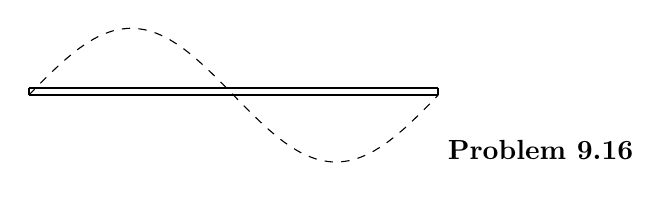
\begin{tikzpicture}[scale=1.0]
  % antenna bar
  \draw[thick] (-2.6,0) -- (2.6,0);
  \draw[thick] (-2.6,0.09) -- (2.6,0.09);
  \draw[thick] (-2.6,0) -- (-2.6,0.09);
  \draw[thick] (2.6,0) -- (2.6,0.09);
  % sinusoidal current distribution: one full wavelength
  \draw[dashed,domain=-2.6:2.6,smooth,variable=\x]
    plot ({\x},{-0.85*sin(360*\x/5.2)});
  \node at (3.9,-0.7) {\textbf{Problem 9.16}};
\end{tikzpicture}
\end{center}

\begin{enumerate}
\item[(a)] Calculate exactly the power radiated per unit solid angle and plot the angular distribution of radiation.
\item[(b)] Determine the total power radiated and find a numerical value for the radiation resistance.
\end{enumerate}
\solution

Use $z$ along the wire and choose the overall current phase so that
$I(z)=I_0\sin(kz)$ on $-d/2<z<d/2$. A full spatial wavelength means
$kd=2\pi$, with $k=\omega/c$. $I_0$ is the \emph{maximum} current
amplitude, not the current at the central node, which is zero.

\textbf{(a)} With $u=\cos\theta$, the exact radiation source integral is
\begin{align*}
F(u)&=\int_{-\pi/k}^{\pi/k}I_0\sin(kz)e^{-ikuz}dz\\
&=-\frac{iI_0}{k}\left[
\frac{\sin[\pi(1-u)]}{1-u}
-\frac{\sin[\pi(1+u)]}{1+u}\right]
=-\frac{2iI_0}{k}\frac{\sin\pi u}{1-u^2}.
\end{align*}
The far vector potential is $\mu_0F(u)\hat{\mathbf z}e^{ikr}/(4\pi r)$.
Its transverse electric field has magnitude
$Z_0k|F|\sin\theta/(4\pi r)$, giving
\[
\boxed{\frac{d\overline P}{d\Omega}
=\frac{Z_0|I_0|^2}{8\pi^2}
\frac{\sin^2(\pi\cos\theta)}{\sin^2\theta}.}
\]
The apparent axial singularities are removable: the expression tends
to zero as $\theta^2$ at either pole. It also vanishes in the equatorial
plane. The polar plot shows the normalized intensity in a meridian;
the dashed curve is the normalized $E2$ pattern used in 9.17.
\begin{center}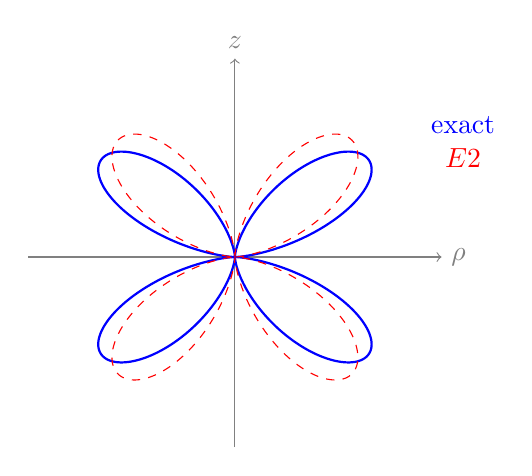
\begin{tikzpicture}[scale=2.1]
\draw[->,gray] (-1.25,0)--(1.25,0) node[right] {$\rho$};
\draw[->,gray] (0,-1.15)--(0,1.2) node[above] {$z$};
\draw[blue,thick] plot coordinates {(0.000000,0.000000) (0.000001,0.000133) (0.000009,0.000531) (0.000031,0.001195) (0.000074,0.002124) (0.000145,0.003319) (0.000250,0.004778) (0.000398,0.006501) (0.000593,0.008487) (0.000845,0.010737) (0.001159,0.013249) (0.001543,0.016022) (0.002003,0.019056) (0.002546,0.022349) (0.003180,0.025901) (0.003911,0.029709) (0.004747,0.033773) (0.005693,0.038091) (0.006757,0.042662) (0.007946,0.047483) (0.009266,0.052553) (0.010725,0.057869) (0.012329,0.063429) (0.014085,0.069231) (0.015999,0.075272) (0.018079,0.081549) (0.020330,0.088059) (0.022759,0.094799) (0.025373,0.101765) (0.028178,0.108954) (0.031179,0.116362) (0.034384,0.123984) (0.037798,0.131817) (0.041427,0.139855) (0.045276,0.148093) (0.049352,0.156526) (0.053660,0.165149) (0.058205,0.173955) (0.062991,0.182939) (0.068024,0.192095) (0.073309,0.201414) (0.078849,0.210891) (0.084649,0.220517) (0.090712,0.230286) (0.097042,0.240188) (0.103642,0.250215) (0.110516,0.260359) (0.117665,0.270610) (0.125091,0.280959) (0.132797,0.291395) (0.140783,0.301910) (0.149050,0.312490) (0.157600,0.323127) (0.166431,0.333808) (0.175543,0.344522) (0.184935,0.355257) (0.194606,0.366000) (0.204552,0.376739) (0.214772,0.387460) (0.225262,0.398150) (0.236018,0.408796) (0.247035,0.419383) (0.258308,0.429897) (0.269831,0.440324) (0.281597,0.450649) (0.293599,0.460858) (0.305828,0.470934) (0.318276,0.480862) (0.330933,0.490628) (0.343788,0.500215) (0.356831,0.509607) (0.370049,0.518790) (0.383430,0.527746) (0.396960,0.536461) (0.410625,0.544918) (0.424410,0.553102) (0.438298,0.560996) (0.452274,0.568586) (0.466319,0.575856) (0.480416,0.582791) (0.494545,0.589376) (0.508687,0.595596) (0.522821,0.601437) (0.536927,0.606885) (0.550982,0.611928) (0.564964,0.616550) (0.578851,0.620741) (0.592618,0.624489) (0.606241,0.627781) (0.619697,0.630608) (0.632959,0.632959) (0.646003,0.634825) (0.658803,0.636198) (0.671332,0.637070) (0.683565,0.637434) (0.695474,0.637285) (0.707035,0.636617) (0.718219,0.635426) (0.729000,0.633710) (0.739352,0.631467) (0.749249,0.628695) (0.758665,0.625395) (0.767574,0.621569) (0.775950,0.617219) (0.783770,0.612348) (0.791009,0.606962) (0.797643,0.601067) (0.803650,0.594670) (0.809008,0.587779) (0.813697,0.580404) (0.817695,0.572556) (0.820985,0.564247) (0.823549,0.555491) (0.825371,0.546301) (0.826435,0.536693) (0.826729,0.526684) (0.826240,0.516292) (0.824959,0.505535) (0.822876,0.494434) (0.819984,0.483008) (0.816279,0.471279) (0.811758,0.459271) (0.806419,0.447005) (0.800263,0.434507) (0.793293,0.421801) (0.785514,0.408913) (0.776932,0.395867) (0.767558,0.382690) (0.757402,0.369410) (0.746479,0.356052) (0.734803,0.342644) (0.722393,0.329213) (0.709269,0.315787) (0.695453,0.302392) (0.680970,0.289055) (0.665847,0.275803) (0.650113,0.262663) (0.633798,0.249660) (0.616935,0.236819) (0.599559,0.224166) (0.581706,0.211724) (0.563416,0.199516) (0.544727,0.187565) (0.525683,0.175891) (0.506325,0.164515) (0.486700,0.153456) (0.466852,0.142731) (0.446829,0.132357) (0.426679,0.122348) (0.406451,0.112719) (0.386194,0.103480) (0.365960,0.094644) (0.345798,0.086217) (0.325761,0.078208) (0.305899,0.070622) (0.286263,0.063463) (0.266906,0.056733) (0.247876,0.050431) (0.229226,0.044557) (0.211004,0.039107) (0.193259,0.034077) (0.176039,0.029459) (0.159391,0.025245) (0.143360,0.021425) (0.127990,0.017988) (0.113322,0.014919) (0.099399,0.012205) (0.086258,0.009828) (0.073936,0.007771) (0.062467,0.006015) (0.051884,0.004539) (0.042217,0.003323) (0.033491,0.002342) (0.025734,0.001574) (0.018965,0.000994) (0.013204,0.000577) (0.008469,0.000296) (0.004772,0.000125) (0.002123,0.000037) (0.000531,0.000005) (0.000000,0.000000) (0.000531,-0.000005) (0.002123,-0.000037) (0.004772,-0.000125) (0.008469,-0.000296) (0.013204,-0.000577) (0.018965,-0.000994) (0.025734,-0.001574) (0.033491,-0.002342) (0.042217,-0.003323) (0.051884,-0.004539) (0.062467,-0.006015) (0.073936,-0.007771) (0.086258,-0.009828) (0.099399,-0.012205) (0.113322,-0.014919) (0.127990,-0.017988) (0.143360,-0.021425) (0.159391,-0.025245) (0.176039,-0.029459) (0.193259,-0.034077) (0.211004,-0.039107) (0.229226,-0.044557) (0.247876,-0.050431) (0.266906,-0.056733) (0.286263,-0.063463) (0.305899,-0.070622) (0.325761,-0.078208) (0.345798,-0.086217) (0.365960,-0.094644) (0.386194,-0.103480) (0.406451,-0.112719) (0.426679,-0.122348) (0.446829,-0.132357) (0.466852,-0.142731) (0.486700,-0.153456) (0.506325,-0.164515) (0.525683,-0.175891) (0.544727,-0.187565) (0.563416,-0.199516) (0.581706,-0.211724) (0.599559,-0.224166) (0.616935,-0.236819) (0.633798,-0.249660) (0.650113,-0.262663) (0.665847,-0.275803) (0.680970,-0.289055) (0.695453,-0.302392) (0.709269,-0.315787) (0.722393,-0.329213) (0.734803,-0.342644) (0.746479,-0.356052) (0.757402,-0.369410) (0.767558,-0.382690) (0.776932,-0.395867) (0.785514,-0.408913) (0.793293,-0.421801) (0.800263,-0.434507) (0.806419,-0.447005) (0.811758,-0.459271) (0.816279,-0.471279) (0.819984,-0.483008) (0.822876,-0.494434) (0.824959,-0.505535) (0.826240,-0.516292) (0.826729,-0.526684) (0.826435,-0.536693) (0.825371,-0.546301) (0.823549,-0.555491) (0.820985,-0.564247) (0.817695,-0.572556) (0.813697,-0.580404) (0.809008,-0.587779) (0.803650,-0.594670) (0.797643,-0.601067) (0.791009,-0.606962) (0.783770,-0.612348) (0.775950,-0.617219) (0.767574,-0.621569) (0.758665,-0.625395) (0.749249,-0.628695) (0.739352,-0.631467) (0.729000,-0.633710) (0.718219,-0.635426) (0.707035,-0.636617) (0.695474,-0.637285) (0.683565,-0.637434) (0.671332,-0.637070) (0.658803,-0.636198) (0.646003,-0.634825) (0.632959,-0.632959) (0.619697,-0.630608) (0.606241,-0.627781) (0.592618,-0.624489) (0.578851,-0.620741) (0.564964,-0.616550) (0.550982,-0.611928) (0.536927,-0.606885) (0.522821,-0.601437) (0.508687,-0.595596) (0.494545,-0.589376) (0.480416,-0.582791) (0.466319,-0.575856) (0.452274,-0.568586) (0.438298,-0.560996) (0.424410,-0.553102) (0.410625,-0.544918) (0.396960,-0.536461) (0.383430,-0.527746) (0.370049,-0.518790) (0.356831,-0.509607) (0.343788,-0.500215) (0.330933,-0.490628) (0.318276,-0.480862) (0.305828,-0.470934) (0.293599,-0.460858) (0.281597,-0.450649) (0.269831,-0.440324) (0.258308,-0.429897) (0.247035,-0.419383) (0.236018,-0.408796) (0.225262,-0.398150) (0.214772,-0.387460) (0.204552,-0.376739) (0.194606,-0.366000) (0.184935,-0.355257) (0.175543,-0.344522) (0.166431,-0.333808) (0.157600,-0.323127) (0.149050,-0.312490) (0.140783,-0.301910) (0.132797,-0.291395) (0.125091,-0.280959) (0.117665,-0.270610) (0.110516,-0.260359) (0.103642,-0.250215) (0.097042,-0.240188) (0.090712,-0.230286) (0.084649,-0.220517) (0.078849,-0.210891) (0.073309,-0.201414) (0.068024,-0.192095) (0.062991,-0.182939) (0.058205,-0.173955) (0.053660,-0.165149) (0.049352,-0.156526) (0.045276,-0.148093) (0.041427,-0.139855) (0.037798,-0.131817) (0.034384,-0.123984) (0.031179,-0.116362) (0.028178,-0.108954) (0.025373,-0.101765) (0.022759,-0.094799) (0.020330,-0.088059) (0.018079,-0.081549) (0.015999,-0.075272) (0.014085,-0.069231) (0.012329,-0.063429) (0.010725,-0.057869) (0.009266,-0.052553) (0.007946,-0.047483) (0.006757,-0.042662) (0.005693,-0.038091) (0.004747,-0.033773) (0.003911,-0.029709) (0.003180,-0.025901) (0.002546,-0.022349) (0.002003,-0.019056) (0.001543,-0.016022) (0.001159,-0.013249) (0.000845,-0.010737) (0.000593,-0.008487) (0.000398,-0.006501) (0.000250,-0.004778) (0.000145,-0.003319) (0.000074,-0.002124) (0.000031,-0.001195) (0.000009,-0.000531) (0.000001,-0.000133) (0.000000,-0.000000) (-0.000001,-0.000133) (-0.000009,-0.000531) (-0.000031,-0.001195) (-0.000074,-0.002124) (-0.000145,-0.003319) (-0.000250,-0.004778) (-0.000398,-0.006501) (-0.000593,-0.008487) (-0.000845,-0.010737) (-0.001159,-0.013249) (-0.001543,-0.016022) (-0.002003,-0.019056) (-0.002546,-0.022349) (-0.003180,-0.025901) (-0.003911,-0.029709) (-0.004747,-0.033773) (-0.005693,-0.038091) (-0.006757,-0.042662) (-0.007946,-0.047483) (-0.009266,-0.052553) (-0.010725,-0.057869) (-0.012329,-0.063429) (-0.014085,-0.069231) (-0.015999,-0.075272) (-0.018079,-0.081549) (-0.020330,-0.088059) (-0.022759,-0.094799) (-0.025373,-0.101765) (-0.028178,-0.108954) (-0.031179,-0.116362) (-0.034384,-0.123984) (-0.037798,-0.131817) (-0.041427,-0.139855) (-0.045276,-0.148093) (-0.049352,-0.156526) (-0.053660,-0.165149) (-0.058205,-0.173955) (-0.062991,-0.182939) (-0.068024,-0.192095) (-0.073309,-0.201414) (-0.078849,-0.210891) (-0.084649,-0.220517) (-0.090712,-0.230286) (-0.097042,-0.240188) (-0.103642,-0.250215) (-0.110516,-0.260359) (-0.117665,-0.270610) (-0.125091,-0.280959) (-0.132797,-0.291395) (-0.140783,-0.301910) (-0.149050,-0.312490) (-0.157600,-0.323127) (-0.166431,-0.333808) (-0.175543,-0.344522) (-0.184935,-0.355257) (-0.194606,-0.366000) (-0.204552,-0.376739) (-0.214772,-0.387460) (-0.225262,-0.398150) (-0.236018,-0.408796) (-0.247035,-0.419383) (-0.258308,-0.429897) (-0.269831,-0.440324) (-0.281597,-0.450649) (-0.293599,-0.460858) (-0.305828,-0.470934) (-0.318276,-0.480862) (-0.330933,-0.490628) (-0.343788,-0.500215) (-0.356831,-0.509607) (-0.370049,-0.518790) (-0.383430,-0.527746) (-0.396960,-0.536461) (-0.410625,-0.544918) (-0.424410,-0.553102) (-0.438298,-0.560996) (-0.452274,-0.568586) (-0.466319,-0.575856) (-0.480416,-0.582791) (-0.494545,-0.589376) (-0.508687,-0.595596) (-0.522821,-0.601437) (-0.536927,-0.606885) (-0.550982,-0.611928) (-0.564964,-0.616550) (-0.578851,-0.620741) (-0.592618,-0.624489) (-0.606241,-0.627781) (-0.619697,-0.630608) (-0.632959,-0.632959) (-0.646003,-0.634825) (-0.658803,-0.636198) (-0.671332,-0.637070) (-0.683565,-0.637434) (-0.695474,-0.637285) (-0.707035,-0.636617) (-0.718219,-0.635426) (-0.729000,-0.633710) (-0.739352,-0.631467) (-0.749249,-0.628695) (-0.758665,-0.625395) (-0.767574,-0.621569) (-0.775950,-0.617219) (-0.783770,-0.612348) (-0.791009,-0.606962) (-0.797643,-0.601067) (-0.803650,-0.594670) (-0.809008,-0.587779) (-0.813697,-0.580404) (-0.817695,-0.572556) (-0.820985,-0.564247) (-0.823549,-0.555491) (-0.825371,-0.546301) (-0.826435,-0.536693) (-0.826729,-0.526684) (-0.826240,-0.516292) (-0.824959,-0.505535) (-0.822876,-0.494434) (-0.819984,-0.483008) (-0.816279,-0.471279) (-0.811758,-0.459271) (-0.806419,-0.447005) (-0.800263,-0.434507) (-0.793293,-0.421801) (-0.785514,-0.408913) (-0.776932,-0.395867) (-0.767558,-0.382690) (-0.757402,-0.369410) (-0.746479,-0.356052) (-0.734803,-0.342644) (-0.722393,-0.329213) (-0.709269,-0.315787) (-0.695453,-0.302392) (-0.680970,-0.289055) (-0.665847,-0.275803) (-0.650113,-0.262663) (-0.633798,-0.249660) (-0.616935,-0.236819) (-0.599559,-0.224166) (-0.581706,-0.211724) (-0.563416,-0.199516) (-0.544727,-0.187565) (-0.525683,-0.175891) (-0.506325,-0.164515) (-0.486700,-0.153456) (-0.466852,-0.142731) (-0.446829,-0.132357) (-0.426679,-0.122348) (-0.406451,-0.112719) (-0.386194,-0.103480) (-0.365960,-0.094644) (-0.345798,-0.086217) (-0.325761,-0.078208) (-0.305899,-0.070622) (-0.286263,-0.063463) (-0.266906,-0.056733) (-0.247876,-0.050431) (-0.229226,-0.044557) (-0.211004,-0.039107) (-0.193259,-0.034077) (-0.176039,-0.029459) (-0.159391,-0.025245) (-0.143360,-0.021425) (-0.127990,-0.017988) (-0.113322,-0.014919) (-0.099399,-0.012205) (-0.086258,-0.009828) (-0.073936,-0.007771) (-0.062467,-0.006015) (-0.051884,-0.004539) (-0.042217,-0.003323) (-0.033491,-0.002342) (-0.025734,-0.001574) (-0.018965,-0.000994) (-0.013204,-0.000577) (-0.008469,-0.000296) (-0.004772,-0.000125) (-0.002123,-0.000037) (-0.000531,-0.000005) (-0.000000,-0.000000) (-0.000531,0.000005) (-0.002123,0.000037) (-0.004772,0.000125) (-0.008469,0.000296) (-0.013204,0.000577) (-0.018965,0.000994) (-0.025734,0.001574) (-0.033491,0.002342) (-0.042217,0.003323) (-0.051884,0.004539) (-0.062467,0.006015) (-0.073936,0.007771) (-0.086258,0.009828) (-0.099399,0.012205) (-0.113322,0.014919) (-0.127990,0.017988) (-0.143360,0.021425) (-0.159391,0.025245) (-0.176039,0.029459) (-0.193259,0.034077) (-0.211004,0.039107) (-0.229226,0.044557) (-0.247876,0.050431) (-0.266906,0.056733) (-0.286263,0.063463) (-0.305899,0.070622) (-0.325761,0.078208) (-0.345798,0.086217) (-0.365960,0.094644) (-0.386194,0.103480) (-0.406451,0.112719) (-0.426679,0.122348) (-0.446829,0.132357) (-0.466852,0.142731) (-0.486700,0.153456) (-0.506325,0.164515) (-0.525683,0.175891) (-0.544727,0.187565) (-0.563416,0.199516) (-0.581706,0.211724) (-0.599559,0.224166) (-0.616935,0.236819) (-0.633798,0.249660) (-0.650113,0.262663) (-0.665847,0.275803) (-0.680970,0.289055) (-0.695453,0.302392) (-0.709269,0.315787) (-0.722393,0.329213) (-0.734803,0.342644) (-0.746479,0.356052) (-0.757402,0.369410) (-0.767558,0.382690) (-0.776932,0.395867) (-0.785514,0.408913) (-0.793293,0.421801) (-0.800263,0.434507) (-0.806419,0.447005) (-0.811758,0.459271) (-0.816279,0.471279) (-0.819984,0.483008) (-0.822876,0.494434) (-0.824959,0.505535) (-0.826240,0.516292) (-0.826729,0.526684) (-0.826435,0.536693) (-0.825371,0.546301) (-0.823549,0.555491) (-0.820985,0.564247) (-0.817695,0.572556) (-0.813697,0.580404) (-0.809008,0.587779) (-0.803650,0.594670) (-0.797643,0.601067) (-0.791009,0.606962) (-0.783770,0.612348) (-0.775950,0.617219) (-0.767574,0.621569) (-0.758665,0.625395) (-0.749249,0.628695) (-0.739352,0.631467) (-0.729000,0.633710) (-0.718219,0.635426) (-0.707035,0.636617) (-0.695474,0.637285) (-0.683565,0.637434) (-0.671332,0.637070) (-0.658803,0.636198) (-0.646003,0.634825) (-0.632959,0.632959) (-0.619697,0.630608) (-0.606241,0.627781) (-0.592618,0.624489) (-0.578851,0.620741) (-0.564964,0.616550) (-0.550982,0.611928) (-0.536927,0.606885) (-0.522821,0.601437) (-0.508687,0.595596) (-0.494545,0.589376) (-0.480416,0.582791) (-0.466319,0.575856) (-0.452274,0.568586) (-0.438298,0.560996) (-0.424410,0.553102) (-0.410625,0.544918) (-0.396960,0.536461) (-0.383430,0.527746) (-0.370049,0.518790) (-0.356831,0.509607) (-0.343788,0.500215) (-0.330933,0.490628) (-0.318276,0.480862) (-0.305828,0.470934) (-0.293599,0.460858) (-0.281597,0.450649) (-0.269831,0.440324) (-0.258308,0.429897) (-0.247035,0.419383) (-0.236018,0.408796) (-0.225262,0.398150) (-0.214772,0.387460) (-0.204552,0.376739) (-0.194606,0.366000) (-0.184935,0.355257) (-0.175543,0.344522) (-0.166431,0.333808) (-0.157600,0.323127) (-0.149050,0.312490) (-0.140783,0.301910) (-0.132797,0.291395) (-0.125091,0.280959) (-0.117665,0.270610) (-0.110516,0.260359) (-0.103642,0.250215) (-0.097042,0.240188) (-0.090712,0.230286) (-0.084649,0.220517) (-0.078849,0.210891) (-0.073309,0.201414) (-0.068024,0.192095) (-0.062991,0.182939) (-0.058205,0.173955) (-0.053660,0.165149) (-0.049352,0.156526) (-0.045276,0.148093) (-0.041427,0.139855) (-0.037798,0.131817) (-0.034384,0.123984) (-0.031179,0.116362) (-0.028178,0.108954) (-0.025373,0.101765) (-0.022759,0.094799) (-0.020330,0.088059) (-0.018079,0.081549) (-0.015999,0.075272) (-0.014085,0.069231) (-0.012329,0.063429) (-0.010725,0.057869) (-0.009266,0.052553) (-0.007946,0.047483) (-0.006757,0.042662) (-0.005693,0.038091) (-0.004747,0.033773) (-0.003911,0.029709) (-0.003180,0.025901) (-0.002546,0.022349) (-0.002003,0.019056) (-0.001543,0.016022) (-0.001159,0.013249) (-0.000845,0.010737) (-0.000593,0.008487) (-0.000398,0.006501) (-0.000250,0.004778) (-0.000145,0.003319) (-0.000074,0.002124) (-0.000031,0.001195) (-0.000009,0.000531) (-0.000001,0.000133) (-0.000000,0.000000)};
\draw[red,dashed] plot coordinates {(0.000000,0.000000) (0.000003,0.000305) (0.000021,0.001218) (0.000072,0.002738) (0.000170,0.004863) (0.000331,0.007589) (0.000572,0.010911) (0.000907,0.014824) (0.001351,0.019322) (0.001920,0.024396) (0.002628,0.030039) (0.003490,0.036240) (0.004518,0.042990) (0.005728,0.050278) (0.007133,0.058090) (0.008744,0.066414) (0.010574,0.075237) (0.012635,0.084542) (0.014938,0.094316) (0.017494,0.104541) (0.020313,0.115201) (0.023404,0.126277) (0.026776,0.137752) (0.030438,0.149606) (0.034396,0.161820) (0.038657,0.174373) (0.043229,0.187244) (0.048115,0.200413) (0.053320,0.213857) (0.058849,0.227554) (0.064705,0.241481) (0.070889,0.255617) (0.077403,0.269936) (0.084248,0.284416) (0.091424,0.299033) (0.098929,0.313763) (0.106763,0.328582) (0.114922,0.343465) (0.123403,0.358388) (0.132202,0.373328) (0.141314,0.388258) (0.150734,0.403156) (0.160454,0.417997) (0.170468,0.432757) (0.180767,0.447413) (0.191342,0.461940) (0.202184,0.476315) (0.213282,0.490515) (0.224626,0.504518) (0.236204,0.518302) (0.248003,0.531843) (0.260010,0.545122) (0.272211,0.558116) (0.284593,0.570806) (0.297141,0.583171) (0.309838,0.595193) (0.322669,0.606853) (0.335618,0.618132) (0.348668,0.629014) (0.361801,0.639481) (0.375000,0.649519) (0.388246,0.659112) (0.401522,0.668245) (0.414808,0.676905) (0.428085,0.685079) (0.441335,0.692757) (0.454537,0.699925) (0.467672,0.706576) (0.480721,0.712699) (0.493664,0.718286) (0.506481,0.723329) (0.519152,0.727824) (0.531657,0.731763) (0.543977,0.735142) (0.556092,0.737958) (0.567982,0.740209) (0.579629,0.741891) (0.591014,0.743006) (0.602117,0.743552) (0.612920,0.743531) (0.623405,0.742945) (0.633555,0.741798) (0.643352,0.740091) (0.652779,0.737832) (0.661820,0.735025) (0.670458,0.731677) (0.678680,0.727795) (0.686469,0.723388) (0.693812,0.718464) (0.700696,0.713033) (0.707107,0.707107) (0.713033,0.700696) (0.718464,0.693812) (0.723388,0.686469) (0.727795,0.678680) (0.731677,0.670458) (0.735025,0.661820) (0.737832,0.652779) (0.740091,0.643352) (0.741798,0.633555) (0.742945,0.623405) (0.743531,0.612920) (0.743552,0.602117) (0.743006,0.591014) (0.741891,0.579629) (0.740209,0.567982) (0.737958,0.556092) (0.735142,0.543977) (0.731763,0.531657) (0.727824,0.519152) (0.723329,0.506481) (0.718286,0.493664) (0.712699,0.480721) (0.706576,0.467672) (0.699925,0.454537) (0.692757,0.441335) (0.685079,0.428085) (0.676905,0.414808) (0.668245,0.401522) (0.659112,0.388246) (0.649519,0.375000) (0.639481,0.361801) (0.629014,0.348668) (0.618132,0.335618) (0.606853,0.322669) (0.595193,0.309838) (0.583171,0.297141) (0.570806,0.284593) (0.558116,0.272211) (0.545122,0.260010) (0.531843,0.248003) (0.518302,0.236204) (0.504518,0.224626) (0.490515,0.213282) (0.476315,0.202184) (0.461940,0.191342) (0.447413,0.180767) (0.432757,0.170468) (0.417997,0.160454) (0.403156,0.150734) (0.388258,0.141314) (0.373328,0.132202) (0.358388,0.123403) (0.343465,0.114922) (0.328582,0.106763) (0.313763,0.098929) (0.299033,0.091424) (0.284416,0.084248) (0.269936,0.077403) (0.255617,0.070889) (0.241481,0.064705) (0.227554,0.058849) (0.213857,0.053320) (0.200413,0.048115) (0.187244,0.043229) (0.174373,0.038657) (0.161820,0.034396) (0.149606,0.030438) (0.137752,0.026776) (0.126277,0.023404) (0.115201,0.020313) (0.104541,0.017494) (0.094316,0.014938) (0.084542,0.012635) (0.075237,0.010574) (0.066414,0.008744) (0.058090,0.007133) (0.050278,0.005728) (0.042990,0.004518) (0.036240,0.003490) (0.030039,0.002628) (0.024396,0.001920) (0.019322,0.001351) (0.014824,0.000907) (0.010911,0.000572) (0.007589,0.000331) (0.004863,0.000170) (0.002738,0.000072) (0.001218,0.000021) (0.000305,0.000003) (0.000000,0.000000) (0.000305,-0.000003) (0.001218,-0.000021) (0.002738,-0.000072) (0.004863,-0.000170) (0.007589,-0.000331) (0.010911,-0.000572) (0.014824,-0.000907) (0.019322,-0.001351) (0.024396,-0.001920) (0.030039,-0.002628) (0.036240,-0.003490) (0.042990,-0.004518) (0.050278,-0.005728) (0.058090,-0.007133) (0.066414,-0.008744) (0.075237,-0.010574) (0.084542,-0.012635) (0.094316,-0.014938) (0.104541,-0.017494) (0.115201,-0.020313) (0.126277,-0.023404) (0.137752,-0.026776) (0.149606,-0.030438) (0.161820,-0.034396) (0.174373,-0.038657) (0.187244,-0.043229) (0.200413,-0.048115) (0.213857,-0.053320) (0.227554,-0.058849) (0.241481,-0.064705) (0.255617,-0.070889) (0.269936,-0.077403) (0.284416,-0.084248) (0.299033,-0.091424) (0.313763,-0.098929) (0.328582,-0.106763) (0.343465,-0.114922) (0.358388,-0.123403) (0.373328,-0.132202) (0.388258,-0.141314) (0.403156,-0.150734) (0.417997,-0.160454) (0.432757,-0.170468) (0.447413,-0.180767) (0.461940,-0.191342) (0.476315,-0.202184) (0.490515,-0.213282) (0.504518,-0.224626) (0.518302,-0.236204) (0.531843,-0.248003) (0.545122,-0.260010) (0.558116,-0.272211) (0.570806,-0.284593) (0.583171,-0.297141) (0.595193,-0.309838) (0.606853,-0.322669) (0.618132,-0.335618) (0.629014,-0.348668) (0.639481,-0.361801) (0.649519,-0.375000) (0.659112,-0.388246) (0.668245,-0.401522) (0.676905,-0.414808) (0.685079,-0.428085) (0.692757,-0.441335) (0.699925,-0.454537) (0.706576,-0.467672) (0.712699,-0.480721) (0.718286,-0.493664) (0.723329,-0.506481) (0.727824,-0.519152) (0.731763,-0.531657) (0.735142,-0.543977) (0.737958,-0.556092) (0.740209,-0.567982) (0.741891,-0.579629) (0.743006,-0.591014) (0.743552,-0.602117) (0.743531,-0.612920) (0.742945,-0.623405) (0.741798,-0.633555) (0.740091,-0.643352) (0.737832,-0.652779) (0.735025,-0.661820) (0.731677,-0.670458) (0.727795,-0.678680) (0.723388,-0.686469) (0.718464,-0.693812) (0.713033,-0.700696) (0.707107,-0.707107) (0.700696,-0.713033) (0.693812,-0.718464) (0.686469,-0.723388) (0.678680,-0.727795) (0.670458,-0.731677) (0.661820,-0.735025) (0.652779,-0.737832) (0.643352,-0.740091) (0.633555,-0.741798) (0.623405,-0.742945) (0.612920,-0.743531) (0.602117,-0.743552) (0.591014,-0.743006) (0.579629,-0.741891) (0.567982,-0.740209) (0.556092,-0.737958) (0.543977,-0.735142) (0.531657,-0.731763) (0.519152,-0.727824) (0.506481,-0.723329) (0.493664,-0.718286) (0.480721,-0.712699) (0.467672,-0.706576) (0.454537,-0.699925) (0.441335,-0.692757) (0.428085,-0.685079) (0.414808,-0.676905) (0.401522,-0.668245) (0.388246,-0.659112) (0.375000,-0.649519) (0.361801,-0.639481) (0.348668,-0.629014) (0.335618,-0.618132) (0.322669,-0.606853) (0.309838,-0.595193) (0.297141,-0.583171) (0.284593,-0.570806) (0.272211,-0.558116) (0.260010,-0.545122) (0.248003,-0.531843) (0.236204,-0.518302) (0.224626,-0.504518) (0.213282,-0.490515) (0.202184,-0.476315) (0.191342,-0.461940) (0.180767,-0.447413) (0.170468,-0.432757) (0.160454,-0.417997) (0.150734,-0.403156) (0.141314,-0.388258) (0.132202,-0.373328) (0.123403,-0.358388) (0.114922,-0.343465) (0.106763,-0.328582) (0.098929,-0.313763) (0.091424,-0.299033) (0.084248,-0.284416) (0.077403,-0.269936) (0.070889,-0.255617) (0.064705,-0.241481) (0.058849,-0.227554) (0.053320,-0.213857) (0.048115,-0.200413) (0.043229,-0.187244) (0.038657,-0.174373) (0.034396,-0.161820) (0.030438,-0.149606) (0.026776,-0.137752) (0.023404,-0.126277) (0.020313,-0.115201) (0.017494,-0.104541) (0.014938,-0.094316) (0.012635,-0.084542) (0.010574,-0.075237) (0.008744,-0.066414) (0.007133,-0.058090) (0.005728,-0.050278) (0.004518,-0.042990) (0.003490,-0.036240) (0.002628,-0.030039) (0.001920,-0.024396) (0.001351,-0.019322) (0.000907,-0.014824) (0.000572,-0.010911) (0.000331,-0.007589) (0.000170,-0.004863) (0.000072,-0.002738) (0.000021,-0.001218) (0.000003,-0.000305) (0.000000,-0.000000) (-0.000003,-0.000305) (-0.000021,-0.001218) (-0.000072,-0.002738) (-0.000170,-0.004863) (-0.000331,-0.007589) (-0.000572,-0.010911) (-0.000907,-0.014824) (-0.001351,-0.019322) (-0.001920,-0.024396) (-0.002628,-0.030039) (-0.003490,-0.036240) (-0.004518,-0.042990) (-0.005728,-0.050278) (-0.007133,-0.058090) (-0.008744,-0.066414) (-0.010574,-0.075237) (-0.012635,-0.084542) (-0.014938,-0.094316) (-0.017494,-0.104541) (-0.020313,-0.115201) (-0.023404,-0.126277) (-0.026776,-0.137752) (-0.030438,-0.149606) (-0.034396,-0.161820) (-0.038657,-0.174373) (-0.043229,-0.187244) (-0.048115,-0.200413) (-0.053320,-0.213857) (-0.058849,-0.227554) (-0.064705,-0.241481) (-0.070889,-0.255617) (-0.077403,-0.269936) (-0.084248,-0.284416) (-0.091424,-0.299033) (-0.098929,-0.313763) (-0.106763,-0.328582) (-0.114922,-0.343465) (-0.123403,-0.358388) (-0.132202,-0.373328) (-0.141314,-0.388258) (-0.150734,-0.403156) (-0.160454,-0.417997) (-0.170468,-0.432757) (-0.180767,-0.447413) (-0.191342,-0.461940) (-0.202184,-0.476315) (-0.213282,-0.490515) (-0.224626,-0.504518) (-0.236204,-0.518302) (-0.248003,-0.531843) (-0.260010,-0.545122) (-0.272211,-0.558116) (-0.284593,-0.570806) (-0.297141,-0.583171) (-0.309838,-0.595193) (-0.322669,-0.606853) (-0.335618,-0.618132) (-0.348668,-0.629014) (-0.361801,-0.639481) (-0.375000,-0.649519) (-0.388246,-0.659112) (-0.401522,-0.668245) (-0.414808,-0.676905) (-0.428085,-0.685079) (-0.441335,-0.692757) (-0.454537,-0.699925) (-0.467672,-0.706576) (-0.480721,-0.712699) (-0.493664,-0.718286) (-0.506481,-0.723329) (-0.519152,-0.727824) (-0.531657,-0.731763) (-0.543977,-0.735142) (-0.556092,-0.737958) (-0.567982,-0.740209) (-0.579629,-0.741891) (-0.591014,-0.743006) (-0.602117,-0.743552) (-0.612920,-0.743531) (-0.623405,-0.742945) (-0.633555,-0.741798) (-0.643352,-0.740091) (-0.652779,-0.737832) (-0.661820,-0.735025) (-0.670458,-0.731677) (-0.678680,-0.727795) (-0.686469,-0.723388) (-0.693812,-0.718464) (-0.700696,-0.713033) (-0.707107,-0.707107) (-0.713033,-0.700696) (-0.718464,-0.693812) (-0.723388,-0.686469) (-0.727795,-0.678680) (-0.731677,-0.670458) (-0.735025,-0.661820) (-0.737832,-0.652779) (-0.740091,-0.643352) (-0.741798,-0.633555) (-0.742945,-0.623405) (-0.743531,-0.612920) (-0.743552,-0.602117) (-0.743006,-0.591014) (-0.741891,-0.579629) (-0.740209,-0.567982) (-0.737958,-0.556092) (-0.735142,-0.543977) (-0.731763,-0.531657) (-0.727824,-0.519152) (-0.723329,-0.506481) (-0.718286,-0.493664) (-0.712699,-0.480721) (-0.706576,-0.467672) (-0.699925,-0.454537) (-0.692757,-0.441335) (-0.685079,-0.428085) (-0.676905,-0.414808) (-0.668245,-0.401522) (-0.659112,-0.388246) (-0.649519,-0.375000) (-0.639481,-0.361801) (-0.629014,-0.348668) (-0.618132,-0.335618) (-0.606853,-0.322669) (-0.595193,-0.309838) (-0.583171,-0.297141) (-0.570806,-0.284593) (-0.558116,-0.272211) (-0.545122,-0.260010) (-0.531843,-0.248003) (-0.518302,-0.236204) (-0.504518,-0.224626) (-0.490515,-0.213282) (-0.476315,-0.202184) (-0.461940,-0.191342) (-0.447413,-0.180767) (-0.432757,-0.170468) (-0.417997,-0.160454) (-0.403156,-0.150734) (-0.388258,-0.141314) (-0.373328,-0.132202) (-0.358388,-0.123403) (-0.343465,-0.114922) (-0.328582,-0.106763) (-0.313763,-0.098929) (-0.299033,-0.091424) (-0.284416,-0.084248) (-0.269936,-0.077403) (-0.255617,-0.070889) (-0.241481,-0.064705) (-0.227554,-0.058849) (-0.213857,-0.053320) (-0.200413,-0.048115) (-0.187244,-0.043229) (-0.174373,-0.038657) (-0.161820,-0.034396) (-0.149606,-0.030438) (-0.137752,-0.026776) (-0.126277,-0.023404) (-0.115201,-0.020313) (-0.104541,-0.017494) (-0.094316,-0.014938) (-0.084542,-0.012635) (-0.075237,-0.010574) (-0.066414,-0.008744) (-0.058090,-0.007133) (-0.050278,-0.005728) (-0.042990,-0.004518) (-0.036240,-0.003490) (-0.030039,-0.002628) (-0.024396,-0.001920) (-0.019322,-0.001351) (-0.014824,-0.000907) (-0.010911,-0.000572) (-0.007589,-0.000331) (-0.004863,-0.000170) (-0.002738,-0.000072) (-0.001218,-0.000021) (-0.000305,-0.000003) (-0.000000,-0.000000) (-0.000305,0.000003) (-0.001218,0.000021) (-0.002738,0.000072) (-0.004863,0.000170) (-0.007589,0.000331) (-0.010911,0.000572) (-0.014824,0.000907) (-0.019322,0.001351) (-0.024396,0.001920) (-0.030039,0.002628) (-0.036240,0.003490) (-0.042990,0.004518) (-0.050278,0.005728) (-0.058090,0.007133) (-0.066414,0.008744) (-0.075237,0.010574) (-0.084542,0.012635) (-0.094316,0.014938) (-0.104541,0.017494) (-0.115201,0.020313) (-0.126277,0.023404) (-0.137752,0.026776) (-0.149606,0.030438) (-0.161820,0.034396) (-0.174373,0.038657) (-0.187244,0.043229) (-0.200413,0.048115) (-0.213857,0.053320) (-0.227554,0.058849) (-0.241481,0.064705) (-0.255617,0.070889) (-0.269936,0.077403) (-0.284416,0.084248) (-0.299033,0.091424) (-0.313763,0.098929) (-0.328582,0.106763) (-0.343465,0.114922) (-0.358388,0.123403) (-0.373328,0.132202) (-0.388258,0.141314) (-0.403156,0.150734) (-0.417997,0.160454) (-0.432757,0.170468) (-0.447413,0.180767) (-0.461940,0.191342) (-0.476315,0.202184) (-0.490515,0.213282) (-0.504518,0.224626) (-0.518302,0.236204) (-0.531843,0.248003) (-0.545122,0.260010) (-0.558116,0.272211) (-0.570806,0.284593) (-0.583171,0.297141) (-0.595193,0.309838) (-0.606853,0.322669) (-0.618132,0.335618) (-0.629014,0.348668) (-0.639481,0.361801) (-0.649519,0.375000) (-0.659112,0.388246) (-0.668245,0.401522) (-0.676905,0.414808) (-0.685079,0.428085) (-0.692757,0.441335) (-0.699925,0.454537) (-0.706576,0.467672) (-0.712699,0.480721) (-0.718286,0.493664) (-0.723329,0.506481) (-0.727824,0.519152) (-0.731763,0.531657) (-0.735142,0.543977) (-0.737958,0.556092) (-0.740209,0.567982) (-0.741891,0.579629) (-0.743006,0.591014) (-0.743552,0.602117) (-0.743531,0.612920) (-0.742945,0.623405) (-0.741798,0.633555) (-0.740091,0.643352) (-0.737832,0.652779) (-0.735025,0.661820) (-0.731677,0.670458) (-0.727795,0.678680) (-0.723388,0.686469) (-0.718464,0.693812) (-0.713033,0.700696) (-0.707107,0.707107) (-0.700696,0.713033) (-0.693812,0.718464) (-0.686469,0.723388) (-0.678680,0.727795) (-0.670458,0.731677) (-0.661820,0.735025) (-0.652779,0.737832) (-0.643352,0.740091) (-0.633555,0.741798) (-0.623405,0.742945) (-0.612920,0.743531) (-0.602117,0.743552) (-0.591014,0.743006) (-0.579629,0.741891) (-0.567982,0.740209) (-0.556092,0.737958) (-0.543977,0.735142) (-0.531657,0.731763) (-0.519152,0.727824) (-0.506481,0.723329) (-0.493664,0.718286) (-0.480721,0.712699) (-0.467672,0.706576) (-0.454537,0.699925) (-0.441335,0.692757) (-0.428085,0.685079) (-0.414808,0.676905) (-0.401522,0.668245) (-0.388246,0.659112) (-0.375000,0.649519) (-0.361801,0.639481) (-0.348668,0.629014) (-0.335618,0.618132) (-0.322669,0.606853) (-0.309838,0.595193) (-0.297141,0.583171) (-0.284593,0.570806) (-0.272211,0.558116) (-0.260010,0.545122) (-0.248003,0.531843) (-0.236204,0.518302) (-0.224626,0.504518) (-0.213282,0.490515) (-0.202184,0.476315) (-0.191342,0.461940) (-0.180767,0.447413) (-0.170468,0.432757) (-0.160454,0.417997) (-0.150734,0.403156) (-0.141314,0.388258) (-0.132202,0.373328) (-0.123403,0.358388) (-0.114922,0.343465) (-0.106763,0.328582) (-0.098929,0.313763) (-0.091424,0.299033) (-0.084248,0.284416) (-0.077403,0.269936) (-0.070889,0.255617) (-0.064705,0.241481) (-0.058849,0.227554) (-0.053320,0.213857) (-0.048115,0.200413) (-0.043229,0.187244) (-0.038657,0.174373) (-0.034396,0.161820) (-0.030438,0.149606) (-0.026776,0.137752) (-0.023404,0.126277) (-0.020313,0.115201) (-0.017494,0.104541) (-0.014938,0.094316) (-0.012635,0.084542) (-0.010574,0.075237) (-0.008744,0.066414) (-0.007133,0.058090) (-0.005728,0.050278) (-0.004518,0.042990) (-0.003490,0.036240) (-0.002628,0.030039) (-0.001920,0.024396) (-0.001351,0.019322) (-0.000907,0.014824) (-0.000572,0.010911) (-0.000331,0.007589) (-0.000170,0.004863) (-0.000072,0.002738) (-0.000021,0.001218) (-0.000003,0.000305) (-0.000000,0.000000)};
\node[blue] at (1.38,.8) {exact};
\node[red] at (1.38,.6) {$E2$};
\end{tikzpicture}
\end{center}

\textbf{(b)} Integration gives
\[
\overline P=\frac{Z_0|I_0|^2}{4\pi}
\int_{-1}^{1}\frac{\sin^2\pi u}{1-u^2}\,du.
\]
By symmetry and partial fractions, the last integral is
\[
\int_{-1}^1\frac{\sin^2\pi u}{1-u}\,du
=\frac12\int_0^{4\pi}\frac{1-\cos t}{t}dt
=\frac12[\gamma_E+\ln(4\pi)-\operatorname{Ci}(4\pi)].
\]
Therefore, defining resistance by $\overline P=R_{\rm rad}|I_0|^2/2$,
\[
\boxed{R_{\rm rad}=\frac{Z_0}{4\pi}
[\gamma_E+\ln(4\pi)-\operatorname{Ci}(4\pi)]
=93.3661\ \Omega.}
\]
This is resistance referred to a current antinode. A feed resistance
referred to the zero central current is not finite in this idealized
prescribed-current model.

\Needspace{5\baselineskip}
\par\bigskip
\noindent\textbf{9.17}\quad Treat the linear antenna of Problem 9.16 by the multipole expansion method.
\begin{enumerate}
\item[(a)] Calculate the multipole moments (electric dipole, magnetic dipole, and electric quadrupole) exactly and in the long-wavelength approximation.
\item[(b)] Compare the shape of the angular distribution of radiated power for the lowest nonvanishing multipole with the exact distribution of Problem 9.16.
\item[(c)] Determine the total power radiated for the lowest multipole and the corresponding radiation resistance using both multipole moments from part a. Compare with Problem 9.16b. Is there a paradox here?
\end{enumerate}
\solution

\textbf{(a)} The source is purely radial along its axis, so
$\mathbf r\times\mathbf J=0$: all magnetic moments vanish exactly.
Because $I(-z)=-I(z)$, continuity gives an even charge density,
$\rho=I'(z)\delta(x)\delta(y)/(i\omega)$; the current vanishes at the
endpoints, so there are no endpoint delta charges. The electric dipole
vanishes by parity, both statically and in the exact dynamic expansion.
The leading electric order is $l=2,m=0$.

For the static, long-wavelength tensor,
\[
Q_{zz}=\frac2{i\omega}\int_{-\pi/k}^{\pi/k}z^2 I'(z)dz
=-\frac4{i\omega}\int zI(z)dz
=\frac{8\pi iI_0}{\omega k^2},\qquad
Q_{xx}=Q_{yy}=-Q_{zz}/2.
\]
Hence $Q_{20}^{\rm LW}=\sqrt{5/(16\pi)}Q_{zz}$.
To calculate the dynamic moment without a long-wavelength expansion,
write $N_l=\sqrt{(2l+1)/(4\pi)}$ and use (9.167). For even $l$ it yields
\[
a_E(l,0)=\frac{2kN_l}{\sqrt{l(l+1)}}\int_0^{\pi/k}
\{-I'[rj_l(kr)]'+k^2rI j_l(kr)\}\,dr.
\]
Integration by parts leaves
\[
\frac{2kN_l}{\sqrt{l(l+1)}}
\left\{-[I'rj_l]_0^{\pi/k}
+\int_0^{\pi/k}rj_l(I''+k^2I)dr\right\}.
\]
The integral is zero for the specified sinusoid, the lower endpoint
vanishes, and $I'(\pi/k)=-kI_0$. Thus
\[
\boxed{a_E(l,0)=kI_0\sqrt{\frac{\pi(2l+1)}{l(l+1)}}j_l(\pi)
\quad(l=2,4,\ldots).}
\]
In particular $j_2(\pi)=3/\pi^2$. Defining an exact effective quadrupole
by $a_E(2,0)=ck^4\sqrt{3/2}\,Q_{20}^{\rm eff}/(15i)$ gives
\[
\boxed{Q_{20}^{\rm eff}=\frac{15}{2\pi^2}Q_{20}^{\rm LW}.}
\]
It is this frequency-dependent moment, not the static integral alone,
that reproduces the entire $l=2$ component at finite $kd$.

\textbf{(b)} Either quadrupole approximation has normalized intensity
proportional to $\sin^2\theta\cos^2\theta$; its maxima are at
$\theta=45^\circ,135^\circ$. The exact pattern is the solid curve in
9.16. Its maxima satisfy
$\pi\cot(\pi u)+u/(1-u^2)=0$, giving
$|u|\simeq0.588981$, or $\theta\simeq53.915^\circ,126.085^\circ$.
The nodes agree, but higher even electric multipoles change the lobes.

\textbf{(c)} Orthogonality of vector spherical harmonics gives
$P_l=Z_0|a_E(l,0)|^2/(2k^2)$. Therefore
\[
\boxed{R_{E2}^{\rm exact}=\frac{15Z_0}{2\pi^3}=91.1260\ \Omega,
\qquad
R_{E2}^{\rm LW}=\frac{2\pi Z_0}{15}=157.8044\ \Omega.}
\]
The exact $E2$ accounts for $97.601\%$ of the $93.3661\ \Omega$ total;
the remaining power is in $l=4,6,\ldots$.
There is no paradox in the long-wavelength estimate exceeding the full
power: $kd=2\pi$ is not small, so that source-size approximation is
uncontrolled. Multipole \emph{order} truncation using the exact coefficient
remains accurate. In particular, inserting $j_2(x)\simeq x^2/15$ into
the boundary-only formula above is not a legitimate way to derive the
static moment: its cancellation used the full Bessel differential
equation and $kd=2\pi$ before the approximation.

\Needspace{5\baselineskip}
\par\bigskip
\noindent\textbf{9.18}\quad A qualitative understanding of the result for the reactance of a short antenna whose radiation fields are described by the electric dipole fields of Section 9.2 can be achieved by considering the idealized dipole fields (9.18).
\begin{enumerate}
\item[(a)] Show that the integral over all angles at fixed distance $r$ of $\epsilon_{0}|\mathbf{E}|^{2}-\mu_{0}|\mathbf{H}|^{2}$ is
\[
\int\left[\epsilon_{0}|\mathbf{E}|^{2}-\mu_{0}|\mathbf{H}|^{2}\right]d\Omega=\frac{1}{2\pi\epsilon_{0}}\frac{|\mathbf{p}|^{2}}{r^{6}}
\]
\item[(b)] Using (6.140) for the reactance, show that the contribution $X_{a}$ to the reactance from fields at distances $r>a$ is
\[
X_{a}=-\frac{\omega}{6\pi\epsilon_{0}}\frac{|\mathbf{p}|^{2}}{|I_{i}|^{2}}\frac{1}{a^{3}}
\]
where $I_{i}$ is the input current.
\item[(c)] For the short center-fed antenna of Section 9.2 show that $X_{a}\simeq-d^{2}/24\pi\epsilon_{0}\omega a^{3}$, corresponding to an effective capacitance $24\pi\epsilon_{0}a^{3}/d^{2}$. With $a=d/2$, $X_{a}$ gives only a small fraction of the total negative reactance of a short antenna. The fields close to the antenna, obviously not dipole in character, contribute heavily. For calculations of reactances of short antennas, see the book by \emph{Schelkunoff and Friis}.
\end{enumerate}
\solution

\textbf{(a)} Put $\mathbf p_T=\mathbf p-\mathbf n(\mathbf n\cdot\mathbf p)$,
$p_n=\mathbf n\cdot\mathbf p$. The exact dipole fields give
\[
E_r=\frac{2p_ne^{ikr}}{4\pi\epsilon_0}
(r^{-3}-ikr^{-2}),\quad
\mathbf E_T=\frac{\mathbf p_Te^{ikr}}{4\pi\epsilon_0}
(k^2r^{-1}+ikr^{-2}-r^{-3}),
\]
\[
\mathbf H=\frac{ce^{ikr}}{4\pi}
(k^2r^{-1}+ikr^{-2})\mathbf n\times\mathbf p.
\]
Since $\mu_0c^2=1/\epsilon_0$, subtraction of the transverse squared
coefficients leaves $r^{-6}-2k^2r^{-4}$, while the radial electric
term contributes $4|p_n|^2(r^{-6}+k^2r^{-4})$.
Use
$\int|p_n|^2d\Omega=4\pi|\mathbf p|^2/3$ and
$\int|\mathbf p_T|^2d\Omega=8\pi|\mathbf p|^2/3$.
The $k^2$ terms cancel, and the $r^{-6}$ coefficient becomes
\[
\boxed{\int(\epsilon_0|\mathbf E|^2-\mu_0|\mathbf H|^2)d\Omega
=\frac{|\mathbf p|^2}{2\pi\epsilon_0r^6}.}
\]

\textbf{(b)} With the reactance convention in (6.140),
\[
X_a=-\frac\omega{|I_i|^2}
\int_a^\infty r^2dr\int(\epsilon_0|\mathbf E|^2-\mu_0|\mathbf H|^2)d\Omega.
\]
As $\int_a^\infty r^{-4}dr=1/(3a^3)$, this yields
$X_a=-\omega|\mathbf p|^2/(6\pi\epsilon_0|I_i|^2a^3)$.
It is negative because the remaining near-field energy is predominantly
electric in this convention.

\textbf{(c)} The short center-fed wire has approximately triangular
current $I(z)=I_i(1-2|z|/d)$, $|z|<d/2$. Continuity gives
$-i\omega p_z=\int I(z)dz=I_id/2$, and thus
$|p_z|^2/|I_i|^2=d^2/(4\omega^2)$. Substitution gives
\[
\boxed{X_a\simeq-\frac{d^2}{24\pi\epsilon_0\omega a^3},\qquad
C_a=\frac{24\pi\epsilon_0a^3}{d^2}.}
\]
For $a=d/2$, $C_a=3\pi\epsilon_0d$. This exterior-field estimate excludes
the strong fields near the wire and gap; it does not determine the full
input reactance of a finite-radius antenna.

\Needspace{5\baselineskip}
\par\bigskip
\noindent\textbf{9.19}\quad Consider the excitation of a waveguide in Problem 8.19 from the point of view of multipole moments of the source.
\begin{enumerate}
\item[(a)] For the linear probe antenna calculate the multipole moment components of $\mathbf{p}$, $\mathbf{m}$, $Q_{\alpha\beta}$, $Q^{M}_{\alpha\beta}$ that enter (9.69).
\item[(b)] Calculate the amplitudes for excitation of the $\mathrm{TE}_{1,0}$ mode and evaluate the power flow. Compare the multipole expansion result with the answer given in Problem 8.19b. Discuss the reasons for agreement or disagreement. What about the comparison for excitation of other modes?
\end{enumerate}
\solution

Use the local origin at the probe's base $(X,0,0)$ and measure $y$ along
it. The mode fields in the expansion are therefore evaluated at that
base. This avoids representing the harmless offset $X$ by extra
translated moments. Write $k_0=\omega/c$, $q=k_0h$, and define
\[
S_j=\int_0^h y^j I_0\sin[k_0(h-y)]dy.
\]
The first two integrals, by elementary integration by parts, are
\[
S_0=\frac{I_0}{k_0}(1-\cos q),\qquad
S_1=I_0\left(\frac h{k_0}-\frac{\sin q}{k_0^2}\right).
\]

\textbf{(a)} Continuity, including injection at the base, gives
$\rho=\partial_y[I(y)\mathbf1_{(0,h)}]/(i\omega)$ times the two
transverse deltas. Integrating its derivative against $y$ and $y^2$
gives
\[
\boxed{\mathbf p=\frac{iS_0}{\omega}\hat{\mathbf y},\quad
\mathbf m=0,\quad
Q=\frac{2iS_1}{\omega}\operatorname{diag}(-1,2,-1),\quad Q^M=0.}
\]
The magnetic moments vanish because $\mathbf r\parallel\mathbf J$ in
these local coordinates. The charge at the base has zero moment but
makes the total oscillating charge zero. For reference, translating the
origin back to the guide corner adds $Q_{xy}=Q_{yx}=3Xp_y$ and
$m_z=XS_0/2$; such translated moments must be used together with a
Taylor expansion about that same corner.

\textbf{(b)} Normalize the transverse mode to unit squared integral,
as in 8.19. For $\mathrm{TE}_{10}$,
\[
E_y(X,y,0)=\sqrt{\frac2{ab}}\sin\frac{\pi X}a,\qquad
Z=\frac{\omega\mu}{k},\quad k^2=k_0^2-(\pi/a)^2.
\]
The quadrupole contraction can be reduced explicitly:
\[
\sum_{ij}Q_{ij}\partial_jE_i
=\frac{2iS_1}{\omega}
(-\partial_xE_x+2\partial_yE_y-\partial_zE_z)
=\frac{6iS_1}{\omega}\partial_yE_y=0.
\]
The second equality uses $\nabla\cdot\mathbf E=0$ and the last uses the
mode's independence of $y$. Equation (9.69) consequently gives
\[
A_{10}^{\pm}=\frac{i\omega Z}{2}\mathbf p\cdot\mathbf E_{10}^{\mp}
=-\frac{ZI_0}{k_0}\sqrt{\frac2{ab}}\sin\frac{\pi X}a
\sin^2\frac{k_0h}{2}.
\]
Its one-direction power is
\[
\boxed{P_+=P_-=
\frac{ZI_0^2}{abk_0^2}\sin^2\frac{\pi X}a\sin^4\frac{k_0h}{2},}
\]
exactly the answer in 8.19. This agreement does not require $k_0h\ll1$:
only $E_y$ enters the source overlap, and it is constant all along the
probe, so the exact integral is already encoded in $\mathbf p$.

For a mode with $n>0$, $E_y\propto\cos(q_ny)$, $q_n=n\pi/b$, and
8.19 contains the different overlap
\[
I_0\frac{k_0[\cos(q_nh)-\cos(k_0h)]}{k_0^2-q_n^2}
=S_0-\frac{q_n^2}{2}S_2+\cdots,
\quad
S_2=I_0\left[\frac{h^2}{k_0}
-\frac{2(1-\cos q)}{k_0^3}\right].
\]
The quadrupole again gives zero because $\partial_yE_y=0$ at the base;
the first omitted coupling is electric octupole order. A dipole
approximation is reliable when the overlap samples $q_nh\ll1$, apart
from cancellations of $S_0$, and not uniformly for high transverse
orders. For $q_n=k_0$ the exact overlap has the removable limit
$I_0h\sin(k_0h)/2$. Modes with $E_y$ identically zero are not excited
at any order by this ideal vertical probe.

\Needspace{5\baselineskip}
\par\bigskip
\noindent\textbf{9.20}\quad\begin{enumerate}
\item[(a)] Verify by direct calculation that the \emph{static} tangential electric field (3.186) in a circular opening in a flat conducting plane, when inserted into the defining equation (9.72) for the electric dipole moment $\mathbf{p}_{\mathrm{eff}}$, leads to the expression (9.75).
\item[(b)] Determine the value of $i\mu\omega\mathbf{m}_{\mathrm{eff}}$ given by (9.72) with the static electric field in part a.
\item[(c)] Use the \emph{static} normal magnetic field (5.132) for the corresponding magnetic boundary problem with a circular opening to compute via (9.74) the magnetic dipole moment $\mathbf{m}_{\mathrm{eff}}$ and compare with (9.75).
\item[(d)] Comment on the differences between the results of parts b and c and the use of the definitions (9.72) in a consistent fashion. [See Section 9 of the article, Diffraction Theory, by C.~J.~B. Bouwkamp in \emph{Reports on Progress in Physics}, Vol.~17, ed. A.~C. Strickland, The Physical Society, London (1954).]
\end{enumerate}
\solution

Take the aperture normal into the region $z>0$ to be
$\mathbf n=\hat{\mathbf z}$ and its radius to be $a$.
In the convention of the static electrostatic solution (3.186), the
asymptotic field in this region is $\mathbf E_0=-E_0\hat{\mathbf z}$;
with zero field on the other side,
\[
\mathbf E_{\rm tan}^{(0)}=\frac{E_0}{\pi}
\frac{\boldsymbol s}{\sqrt{a^2-s^2}},\quad 0<s<a.
\]
If both sides have imposed fields, replace $E_0$ by the corresponding
scalar difference. This sign convention is important in comparing
with (9.75).

\textbf{(a)} The required radial integral is
\[
\int_0^a\frac{s^3}{\sqrt{a^2-s^2}}ds
=a^3\int_0^{\pi/2}\sin^3u\,du=\frac{2a^3}{3}.
\]
Hence
\[
\mathbf p_{\rm eff}=\epsilon_0\hat{\mathbf z}\int
\boldsymbol s\cdot\mathbf E_{\rm tan}^{(0)}d^2s
=\frac{4\epsilon_0a^3E_0}{3}\hat{\mathbf z}
=\boxed{-\frac{4\epsilon_0a^3}{3}\mathbf E_0}.
\]

\textbf{(b)} The other definition gives
\[
i\mu\omega\mathbf m_{\rm eff}
=2\int\mathbf n\times\mathbf E_{\rm tan}^{(0)}d^2s=0,
\]
because the angular integral of $\hat{\boldsymbol\phi}$ is zero.
This calculation uses only the electrostatic part of the aperture field.

\textbf{(c)} For an imposed $\mathbf H_0=H_0\hat{\mathbf y}$ in the
same upper region, the static magnetic solution (5.132) is
$H_z=2H_0s\sin\phi/[\pi\sqrt{a^2-s^2}]$.
Thus
\[
\mathbf m_{\rm eff}=2\int\boldsymbol s H_zd^2s
=\frac{4H_0}{\pi}\frac{2a^3}{3}
\int_0^{2\pi}(\hat{\mathbf x}\cos\phi+
\hat{\mathbf y}\sin\phi)\sin\phi\,d\phi
=\boxed{\frac{8a^3}{3}\mathbf H_0}.
\]
Reversing the observation side reverses the effective moments for fixed
aperture fields, consistently with the normal in their definitions.

\textbf{(d)} There is no inconsistency between the two exact definitions.
For a harmonic Maxwell field, integration by parts in the aperture and
$\nabla_t\times\mathbf E_t=i\omega\mu H_n$ give
\[
\int\mathbf n\times\mathbf E_t\,d^2s
=\int\boldsymbol s(\nabla_t\times\mathbf E_t)_n\,d^2s
=i\omega\mu\int\boldsymbol sH_n\,d^2s.
\]
The boundary term is zero because the electric field tangent to the
rim is zero; the integrable inverse-square-root edge singularity does
not alter it. In a low-frequency expansion
$\mathbf E_t=\mathbf E_t^{(0)}+\omega\mathbf E_t^{(1)}+\cdots$,
the first term determines $\mathbf p_{\rm eff}$, but its curl and its
integrated cross product vanish. The explicit $1/\omega$ in the magnetic
definition promotes $\omega\mathbf E_t^{(1)}$ to a finite leading term.
One must retain that inductive electric field, or equivalently use the
static magnetic solution in (9.74). The electric and magnetic static
boundary problems specify independent leading excitations; setting the
former equal to the entire finite-frequency field loses the latter.

\Needspace{5\baselineskip}
\par\bigskip
\noindent\textbf{9.21}\quad The fields representing a transverse magnetic wave propagating in a cylindrical waveguide of radius $R$ are:
\begin{align*}
E_{z}&=J_{m}(\gamma r)e^{im\phi}e^{i\beta z-i\omega t},\qquad H_{z}=0\\[4pt]
E_{\phi}&=\frac{-m\beta}{\gamma^{2}}\frac{E_{z}}{r},\qquad\qquad\; H_{r}=-\frac{k}{Z_{0}\beta}\,E_{\phi}\\[4pt]
E_{r}&=\frac{i\beta}{\gamma^{2}}\frac{\partial E_{z}}{\partial r},\qquad\qquad\quad H_{\phi}=\frac{k}{Z_{0}\beta}\,E_{r}
\end{align*}
where $m$ is the index specifying the angular dependence, $\beta$ is the propagation constant, $\gamma^{2}=k^{2}-\beta^{2}$ ($k=\omega/c$), where $\gamma$ is such that $J_{m}(\gamma R)=0$. Calculate the ratio of the $z$ component of the electromagnetic angular momentum to the energy in the field. It may be advantageous to perform some integrations by parts, and to use the differential equation satisfied by $E_{z}$, to simplify your calculations.
\solution

All energies and angular momenta below are time averages per unit length.
Let $\psi=J_m(\gamma r)e^{im\phi}$ and
$N=\int_{r<R}|\psi|^2dA$.
The transverse Helmholtz equation and $\psi(R)=0$ imply, by integration
by parts with the vanishing boundary term,
\[
\int|\nabla_t\psi|^2dA=-\int\psi^*\nabla_t^2\psi\,dA=\gamma^2N.
\]
Consequently the field expressions in the question give
\[
\int|\mathbf E_t|^2dA=\frac{\beta^2}{\gamma^2}N,
\qquad
\int|\mathbf H_t|^2dA=\frac{k^2}{Z_0^2\gamma^2}N.
\]
Since $\mu_0/Z_0^2=\epsilon_0$ and $k^2=\beta^2+\gamma^2$,
\[
\frac UL=\frac14\int(\epsilon_0|\mathbf E|^2+
\mu_0|\mathbf H|^2)dA
=\frac{\epsilon_0N}{4}
\left[1+\frac{\beta^2+k^2}{\gamma^2}\right]
=\frac{\epsilon_0k^2N}{2\gamma^2}.
\]
The angular momentum density is
$\mathbf r\times\operatorname{Re}(\mathbf E\times\mathbf H^*)/(2c^2)$.
Here $(\mathbf E\times\mathbf H^*)_\phi=E_zH_r^*$ and
$H_r=km\psi/(Z_0\gamma^2r)$. Therefore
\[
\frac{L_z}{L}=\frac1{2c^2}\int r\operatorname{Re}(E_zH_r^*)dA
=\frac{mkN}{2c^2Z_0\gamma^2}.
\]
Dividing and using $\epsilon_0Z_0=1/c$ gives
\[
\boxed{\frac{L_z}{U}=\frac{m}{ck}=\frac m\omega.}
\]
The sign is that of the helical angular phase $e^{im\phi}$.
A real standing angular pattern such as $\cos m\phi$ combines equal
$+m$ and $-m$ waves and has zero net $L_z$, despite the same energy.

\Needspace{5\baselineskip}
\par\bigskip
\noindent\textbf{9.22}\quad A spherical hole of radius $a$ in a conducting medium can serve as an electromagnetic resonant cavity.
\begin{enumerate}
\item[(a)] Assuming infinite conductivity, determine the transcendental equations for the characteristic frequencies $\omega_{lm}$ of the cavity for TE and TM modes.
\item[(b)] Calculate numerical values for the wavelength $\lambda_{lm}$ in units of the radius $a$ for the four lowest modes for TE and TM waves.
\item[(c)] Calculate explicitly the electric and magnetic fields inside the cavity for the lowest TE and lowest TM mode.
\end{enumerate}
\solution

\textbf{(a)} A regular spherical wave has radial function $j_l(kr)$,
$l\ge1$. With normalized vector harmonic
$\mathbf X_{lm}=\mathbf L Y_{lm}/\sqrt{l(l+1)}$,
where $\mathbf L=-i\mathbf r\times\nabla$ as in (9.101), TE modes have
$\mathbf E\propto j_l(kr)\mathbf X_{lm}$ and TM modes have
$\mathbf H\propto j_l(kr)\mathbf X_{lm}$. Curling the latter gives a
tangential electric field proportional to $[xj_l(x)]'/x$.
The perfectly conducting boundary therefore requires
\[
\boxed{j_l(x_{ln}^{\rm TE})=0,\qquad
[xj_l(x)]'_{x=x_{ln}^{\rm TM}}=0,\qquad
\omega_{ln}=cx_{ln}/a.}
\]
Here $n=1,2,\ldots$ counts positive radial roots; it is distinct from
the azimuthal index $m=-l,\ldots,l$. Every listed frequency has
$2l+1$ angular degeneracy. There is no nonzero-frequency $l=0$
electromagnetic cavity mode.

\textbf{(b)} Root bracketing and refinement give the four lowest
\emph{distinct frequencies} in each family:
\begin{center}
\begin{tabular}{ccrr}
\toprule
Family&$(l,n)$&$x=\omega a/c$&$\lambda/a=2\pi/x$\\
\midrule
TE&$(1,1)$&4.493409458&1.398311319\\
TE&$(2,1)$&5.763459197&1.090176072\\
TE&$(3,1)$&6.987932001&0.899148032\\
TE&$(1,2)$&7.725251837&0.813330807\\
TM&$(1,1)$&2.743707270&2.290034865\\
TM&$(2,1)$&3.870238580&1.623462011\\
TM&$(3,1)$&4.973420351&1.263352957\\
TM&$(4,1)$&6.061949363&1.036495842\\
\bottomrule
\end{tabular}
\end{center}
The supplementary calculation searches several $l$ and radial roots
before sorting, so the TE fourth entry is not incorrectly identified
with $(4,1)$.

\textbf{(c)} Choose the $m=0$ member; rotations and complex linear
combinations produce the other members of each lowest $l=1$ triplet.
Let $x=kr$, $j=j_1(x)$, and $D=[xj_1(x)]'$.
An explicit TE field with arbitrary amplitude $E_*$ is
\[
\boxed{E_\phi=E_*j\sin\theta,\quad
H_r=\frac{2E_*}{i\omega\mu_0r}j\cos\theta,\quad
H_\theta=-\frac{E_*}{i\omega\mu_0r}D\sin\theta,}
\]
with other components zero and $ka=4.493409458$.
These follow directly from
$(\nabla\times\mathbf E)_r=(r\sin\theta)^{-1}
\partial_\theta(\sin\theta E_\phi)$ and
$(\nabla\times\mathbf E)_\theta=-r^{-1}\partial_r(rE_\phi)$,
using $\nabla\times\mathbf E=i\omega\mu_0\mathbf H$.
For the TM mode, choose an arbitrary $H_*$ and use
$\nabla\times\mathbf H=-i\omega\epsilon_0\mathbf E$:
\[
\boxed{H_\phi=H_*j\sin\theta,\quad
E_r=-\frac{2H_*}{i\omega\epsilon_0r}j\cos\theta,\quad
E_\theta=\frac{H_*}{i\omega\epsilon_0r}D\sin\theta,}
\]
with $ka=2.743707270$. The limits at the origin are finite because
$j_1(x)\sim x/3$ and $D\sim2x/3$. The respective conditions $j(ka)=0$
and $D(ka)=0$ make the wall's tangential electric field vanish.

\Needspace{5\baselineskip}
\par\bigskip
\noindent\textbf{9.23}\quad The spherical resonant cavity of Problem 9.22 has nonpermeable walls of large, but finite, conductivity. In the approximation that the skin depth $\delta$ is small compared to the cavity radius $a$, show that the $Q$ of the cavity, defined by equation (8.86), is given by
\begin{align*}
Q&=\frac{a}{\delta}\hspace{3.6cm}\text{for all TE modes}\\[4pt]
Q&=\frac{a}{\delta}\left(1-\frac{l(l+1)}{x_{lm}^{2}}\right)\qquad\text{for TM modes}
\end{align*}
where $x_{lm}=(a/c)\omega_{lm}$ for TM modes.
\solution

For a good nonmagnetic conductor,
$R_s=1/(\sigma\delta)=\omega\mu_0\delta/2$.
The leading wall dissipation is
$P_{\rm loss}=(R_s/2)\int_{r=a}|\mathbf H_t|^2dA$.
Electric and magnetic stored energies are equal in a lossless cavity,
so its total time-averaged energy is
$U=(\mu_0/2)\int|\mathbf H|^2dV$. Thus
\[
Q=\frac{\omega U}{P_{\rm loss}}
=\frac2\delta\frac{\int|\mathbf H|^2dV}
{\int_{r=a}|\mathbf H_t|^2dA}.
\]
Let $x=ka$ and $I_l=\int_0^a r^2j_l(kr)^2dr$. Multiplying the spherical
Bessel equation by its solution, or differentiating its adjacent-order
recurrences, gives
\[
I_l=\frac{a^3}{2}[j_l(x)^2-j_{l-1}(x)j_{l+1}(x)].
\]
To verify the integral rather than assume it, put $j=j_l(x)$ and
use $j_{l-1}=j'+(l+1)j/x$, $j_{l+1}=lj/x-j'$. The proposed
dimensionless antiderivative is
\[
F(x)=\frac{x^3}{2}(j^2+j'^2)+\frac{x^2}{2}jj'
-\frac{l(l+1)x}{2}j^2.
\]
Differentiation gives
\begin{align*}
F'={}&\frac{3x^2}{2}(j^2+j'^2)+x^3(jj'+j'j'')
+xjj'+\frac{x^2}{2}(j'^2+jj'')\\
&-\frac{l(l+1)}2j^2-l(l+1)xjj'.
\end{align*}
Substituting $j''=-2j'/x-[1-l(l+1)/x^2]j$ cancels all $jj'$
and $j'^2$ terms and leaves $F'=x^2j^2$. Integrating from zero to
$ka$ and dividing by $k^3$ proves the identity; its lower endpoint
vanishes since $l\ge1$.

For TM modes $\mathbf H=H_*j_l(kr)\mathbf X_{lm}$, with
$\int|\mathbf X_{lm}|^2d\Omega=1$, so the ratio of integrals is
$I_l/[a^2j_l(x)^2]$. The condition $j_l+xj_l'=0$ and the recurrences give
$j_{l-1}=lj_l/x$, $j_{l+1}=(l+1)j_l/x$. Hence
\[
\boxed{Q_{\rm TM}=\frac a\delta
\left[1-\frac{l(l+1)}{x^2}\right].}
\]

For TE modes take $\mathbf E=E_*j_l\mathbf X_{lm}$.
After curling, the angularly integrated magnetic norm is proportional to
$\int_0^a\{l(l+1)j_l^2+[(rj_l)']^2\}dr$.
For the integration by parts, set $y(r)=rj_l(kr)$. Its equation is
$y''+[k^2-l(l+1)/r^2]y=0$, so
\[
\int_0^a(y')^2dr=[yy']_0^a-\int_0^a yy''dr
=[yy']_0^a+k^2\int_0^a y^2dr
-l(l+1)\int_0^a\frac{y^2}{r^2}dr.
\]
The last term cancels the other term in the magnetic norm. The result is
$k^2I_l+[rj_l(rj_l)']_0^a=k^2I_l$ at the TE root $j_l(x)=0$.
The surface norm has the same common factor times $[xj_l'(x)]^2$.
At this root $j_{l-1}=j_l'$ and $j_{l+1}=-j_l'$, so
$I_l=a^3j_l'^2/2$. Consequently
\[
\boxed{Q_{\rm TE}=\frac2\delta
\frac{k^2a^3j_l'^2/2}{x^2j_l'^2}=\frac a\delta.}
\]
The skin depth is evaluated at the mode frequency. Corrections to these
expressions are beyond leading order in $\delta/a$; the lossless mode
fields suffice at this order.

\Needspace{5\baselineskip}
\par\bigskip
\noindent\textbf{9.24}\quad Discuss the normal modes of oscillation of a perfectly conducting solid sphere of radius $a$ in free space. (This problem was solved by J.~J. Thomson in the 1880s.)
\begin{enumerate}
\item[(a)] Determine the characteristic equations for the eigenfrequencies for TE and TM modes of oscillation. Show that the roots for $\omega$ always have a negative imaginary part, assuming a time dependence of $e^{-i\omega t}$.
\item[(b)] Calculate the eigenfrequencies for the $l=1$ and $l=2$ TE and TM modes. Tabulate the wavelength (defined in terms of the real part of the frequency) in units of the radius $a$ and the decay time (defined as the time taken for the \emph{energy} to fall to $e^{-1}$ of its initial value) in units of the transit time $(a/c)$ for each of the modes.
\end{enumerate}
\solution

\textbf{(a)} Exterior natural oscillations obey an outgoing condition,
so replace the regular $j_l$ of 9.22 by $h_l^{(1)}$. With $x=\omega a/c$,
\[
\boxed{h_l^{(1)}(x)=0\quad({\rm TE}),\qquad
[xh_l^{(1)}(x)]'=0\quad({\rm TM}),\qquad l\ge1.}
\]
These are radiative resonances, not the real eigenfrequencies of a closed
cavity. To exclude $\operatorname{Im}\omega>0$, note that an outgoing
field would then decay exponentially at infinity. Integrating
$\nabla\cdot(\mathbf E\times\mathbf H^*)=
 i\omega\mu_0|\mathbf H|^2-i\omega^*\epsilon_0|\mathbf E|^2$
over the exterior and taking the real part gives
\[
0=-\operatorname{Im}\omega\int
(\mu_0|\mathbf H|^2+\epsilon_0|\mathbf E|^2)dV.
\]
The PEC surface has no normal energy flow and the outer surface term
vanishes, so a nonzero mode is impossible in that half-plane.
For real nonzero $\omega$, outgoing radiation instead has strictly
positive power at infinity, again incompatible with a source-free PEC
boundary. Thus all nonzero radiative roots have
$\operatorname{Im}\omega<0$. Static exterior charge or magnetic fields
at $\omega=0$ are separate boundary-value solutions, not these oscillatory
radiation modes.

\textbf{(b)} The explicit outgoing functions are
\[
h_1^{(1)}(x)=-\frac{e^{ix}}{x^2}(x+i),\qquad
h_2^{(1)}(x)=\frac{ie^{ix}}{x^3}(x^2+3ix-3).
\]
Thus TE roots are $x=-i$ for $l=1$ and
$x=\pm\sqrt3/2-3i/2$ for $l=2$.
Differentiating $xh_l$ gives the TM polynomials
\[
l=1:\quad x^2+ix-1=0,
\qquad
l=2:\quad x^3+3ix^2-6x-6i=0.
\]
The first gives $x=\pm\sqrt3/2-i/2$.
For the cubic put $x=-iy$; it becomes
$y^3-3y^2+6y-6=0$. With
\[
b=1+\sqrt[3]{1+\sqrt2}+\sqrt[3]{1-\sqrt2}=1.596071638,
\]
its roots in $x$ are
\[
x=-ib,\qquad
x=\pm\frac12\sqrt{3b^2-6b+15}
-\frac i2(3-b)
=\pm1.807339494-0.701964181i.
\]
For each root the local field amplitude varies as
$e^{\operatorname{Im}\omega t}$ and its energy as
$e^{2\operatorname{Im}\omega t}$. Therefore
$\tau_E/(a/c)=-1/(2\operatorname{Im}x)$ and
$\lambda/a=2\pi/|\operatorname{Re}x|$ when the real part is nonzero:
\begin{center}
\begin{tabular}{ccrr}
\toprule
Family&$x=\omega a/c$&$\lambda/a$&$\tau_E/(a/c)$\\
\midrule
TE, $l=1$&$-i$&$\infty$ (no oscillation)&0.500000\\
TM, $l=1$&$\pm0.866025404-0.5i$&7.255197457&1.000000\\
TE, $l=2$&$\pm0.866025404-1.5i$&7.255197457&0.333333\\
TM, $l=2$&$-1.596071638i$&$\infty$ (no oscillation)&0.313269\\
TM, $l=2$&$\pm1.807339494-0.701964181i$&3.476483&0.712287\\
\bottomrule
\end{tabular}
\end{center}
Each row also has the usual $2l+1$ angular degeneracy. Negative-real-part
partners supply the reality-related time dependence, rather than new
positive-frequency resonances. The outgoing resonance functions grow
spatially at infinity for these complex frequencies, so a single such
mode is not a finite-total-energy field on all of space at one time.
The stated decay time describes the ringing field in a fixed bounded
exterior region; a causal physical signal includes its propagating front.
